\documentclass[11pt]{article}
\usepackage[T1]{fontenc}
\usepackage{lmodern,microtype}
\usepackage[margin=1.05in]{geometry}
\usepackage{amsmath,amssymb,amsthm,mathtools}
\usepackage{enumitem,booktabs,longtable,array}
\usepackage{xcolor,tikz}
\usetikzlibrary{arrows.meta,positioning,calc,fit,decorations.pathreplacing}
\usepackage[colorlinks=true,linkcolor=blue!45!black,citecolor=blue!45!black,urlcolor=blue!45!black]{hyperref}
\newtheorem{theorem}{Theorem}[section]
\newtheorem{proposition}[theorem]{Proposition}
\newtheorem{lemma}[theorem]{Lemma}
\newtheorem{corollary}[theorem]{Corollary}
\theoremstyle{definition}
\newtheorem{definition}[theorem]{Definition}
\theoremstyle{remark}
\newtheorem{remark}[theorem]{Remark}
\DeclareMathOperator{\diam}{diam}
\DeclareMathOperator{\id}{id}
\DeclareMathOperator{\sht}{ht}
\setlist{itemsep=3pt,topsep=5pt}
\numberwithin{equation}{section}
\pdftrailerid{}
\title{Finite Monoid Computations and a Uniform Generalized Star-Height Bound}
\author{OpenAI}
\date{September 25, 2026}
\hypersetup{
  pdftitle={Finite Monoid Computations and a Uniform Generalized Star-Height Bound},
  pdfauthor={OpenAI}
}
\begin{document}
\maketitle
\begin{abstract}
Every regular language over a finite alphabet has a generalized regular
expression of star height at most thirteen over that same alphabet.
We prove this uniform bound by representing finite monoid computations as
affine updates and recovering them through twelve successive split
constructions.
\end{abstract}
\section{Introduction}\label{sec:introduction}

The generalized star-height problem asks how much nested iteration is
needed to describe regular languages when complement is available.
Complement can replace some uses of iteration, but its presence does not
make ordinary star-height arguments applicable: a lower bound proved for
expressions without complement need not survive its addition. Our aim is
an absolute bound, independent of the alphabet and of the recognizing
automaton, obtained from a fixed number of operations on finite computations.

A generalized regular expression over a finite alphabet \(\Sigma\) is formed
from \(0,1\), and the letters of \(\Sigma\), using union, concatenation,
complement, and Kleene star. The constants denote the empty language and
\(\{\epsilon\}\), and a letter denotes its singleton language. Every
complement is relative to the same \(\Sigma^*\). Define the height by
\[
\begin{aligned}
 \sht(0)=\sht(1)=\sht(a)&=0,\\
 \sht(P+Q)=\sht(PQ)&=\max\{\sht(P),\sht(Q)\},\\
 \sht(\neg P)&=\sht(P),&
 \sht(P^*)&=\sht(P)+1.
\end{aligned}
\]
For a regular language \(L\subseteq\Sigma^*\), let \(h_\Sigma(L)\) be the
minimum of these heights among expressions denoting \(L\). Here regular
means accepted by a deterministic finite automaton (DFA), with a finite
state set, letter transitions, an initial state, and accepting states.
There is no restriction on expression length. The uniform-boundedness question asks
whether one integer bounds \(h_\Sigma(L)\) for every finite \(\Sigma\) and
every regular \(L\) over it. These conventions agree with the standard
Boolean expression model in \cite[\S1]{PST1992}.

\begin{theorem}\label{thm:main}
For every finite alphabet \(\Sigma\) and every regular language
\(L\subseteq\Sigma^*\),
\[
                         h_\Sigma(L)\le 13.
\]
\end{theorem}

This gives an affirmative answer to uniform boundedness. It does not settle
whether height one always suffices. Straubing explicitly distinguishes
these two questions~\cite[p.~537]{Straubing2002}: a language requiring
height greater than one would rule out the bound one, but would not rule
out a larger absolute bound. Computing the minimum generalized height of
a given language is a further question. The construction below supplies
a uniform upper bound; it does not determine that minimum.

The complete construction below uses prediction trials and full decision
histories. Two separate companion articles prove the smaller bounds
four~\cite[Theorem~1.1]{OpenAIHeight4} and
three~\cite[Theorem~1.1]{OpenAIHeight3}, respectively by multiscale
periodic transport and by arbitrary-function shift tables with a
whole-stencil decoder. Each article proves its own needed local statements.
Here the value thirteen records the depth of the prediction/history method;
the stronger numerical bounds do not replace any step of its proof.

\subsection*{Historical and algebraic context}

Eggan related ordinary star height to transition graphs~\cite{Eggan1963},
and Dejean and Sch\"utzenberger gave ordinary-height examples over a
binary alphabet~\cite{DejeanSchutzenberger1966}. Their expressions omit
complement, so their lower bounds do not transfer to the generalized
model. The effect of complement already appears at height zero:
\(\Sigma^*=\neg0\) is star-free. Sch\"utzenberger's 1965 theorem
characterizes the star-free languages as those recognized by finite
aperiodic monoids~\cite{Schutzenberger1965}. Here a finite monoid is
aperiodic if each element \(x\) satisfies \(x^n=x^{n+1}\) for some \(n\).

This characterization makes finite monoids a natural setting for the
problem. A word acts on the states of a DFA, and the induced
transformations form a finite monoid under composition. Height-one
results cover several algebraic classes. Henneman's
result for finite abelian groups is recalled and proved by Pin,
Straubing, and Th\'erien~\cite[Theorem~3.4]{PST1992}; their own
Theorem~7.3 establishes height at most one for languages recognized by
finite nilpotent groups of class two. Bourne and Ru\v{s}kuc subsequently
proved the same bound for languages recognized by finite Rees
zero-matrix semigroups over abelian
groups~\cite[Theorem~3.6]{BourneRuskuc2016}. These results treat specified
recognizing classes; the construction here applies to every finite
transition monoid.

The alphabet and morphism conventions are essential to this comparison.
Pin, Straubing, and Th\'erien prove that star-free injective substitutions
and inverse alphabetic morphisms do not increase generalized
height~\cite[Theorem~4.6 and Corollary~4.7]{PST1992}. Their Theorem~8.1
also represents every regular language as an inverse image, under a
general morphism, of a language of ordinary height at most one. The
inverse-image closure above is restricted to alphabetic morphisms, so it
does not turn this representation into a height-one theorem. Our proof
constructs every expression directly over the original alphabet.

Place and Zeitoun's 2017 account distinguishes the ordinary and
generalized problems and records that no language of generalized height
greater than one was then known~\cite[\S1]{PlaceZeitoun2017}.
Cotumaccio's February 2025 discussion still identifies generalized star
height as an open problem connected with automata and
compression~\cite[p.~46]{Cotumaccio2025}. The theorem above addresses
uniform boundedness; the two stronger companion bounds stated earlier
also do not settle whether height one suffices.

The local-marker ingredient comes from a different tradition. Krieger's
separated-marker construction~\cite[Lemma~2]{Krieger1982} places markers
apart while controlling markerless regions by periodicity. Meyerovitch
presents a clopen-marker form and its finite merging
argument~\cite[\S3, Lemmas~3.2--3.4]{Meyerovitch2025}. Section~\ref{sec:geometry}
proves the precise finite-window construction and periodicity estimates
needed here. The historical results provide context; every local lemma
used to obtain the bound thirteen is proved below.

\subsection*{The mechanism of the proof}

Fix the finite monoid of a recognizing DFA. We represent its action on a
finite vector space over \(\mathbf F_2\). A word will be parsed into
nonempty pieces, called episodes, and one final remainder. The episodes
form a prefix code: no episode is a proper prefix of another. Consequently
their parsing is unique. Each episode carries a total finite-state update.
A graph language specifies the initial and final states of the composed
update on an episode sequence.

The basic step splits an episode into a prefix and a suffix. The prefix
checks the incoming state and the suffix checks the outgoing state. Each
side may choose its own finite metadata. For soundness, every pair of
successful choices must describe the actual episode update and consume
exactly one episode. For availability, every designated episode and every
input state must admit some successful cut. If graph languages for the
remaining episodes are already known, one additional star combines their
sequences with the successful splits. Lemma~\ref{lem:split} states this
identity and its exact height cost.

Three constructions make a bounded number of these steps sufficient.
\begin{enumerate}[leftmargin=*,label=\textup{\arabic*.}]
\item \emph{An affine computation tolerates a controlled disagreement.}
A map \(v\mapsto vA+b\) has linear part \(A\), which is recovered
from its values at \(v\) and at zero. Our finite clock ensures that,
at a given total length residue, independently successful tags either
agree or have one fixed off-diagonal pair. In the latter case the
claimed input and output fit one affine correction with the required
linear part. The clock also bounds how many ordered pairs of candidate
cuts are spoiled, independently of the size of their finite roster.
\item \emph{Prediction and periodicity handle two large episode classes.}
A trial predicts the monoid products on a fixed subdivision and offers
one block of cuts for each input--output vector pair. Partial prefix
and suffix checks always fit a deterministic affine trial update;
a perfect prediction supplies a cut for every input. Local markers
select the trial boundaries. When a boundary window is markerless,
periodicity supplies a second family of cuts with a constant monoid
prefix product and constant context. These are the two outer splits.
\item \emph{Five residual witnesses permit exact time decoding.}
Failure of the two availability conditions has one of five explicit
types. At each type we place many copies of every required cut kind.
A suffix checks all candidate origins and identifies the unique one
having the current witness after later witnesses have been excluded.
A bound on ambiguous ordered pairs leaves a usable copy of each kind.
One aligned split then uses a perfect trial. If the actual full decision
history has no perfect trial, a second split recovers a measurement
from that history. Both splits compute the same affine update on a
larger space; its linear part encodes the target update and resets an
auxiliary monoid register, so the encoding composes across episodes.
The argument counts all leaves, including those that no actual prefix
can realize; it never cancels a monoid factor.
\end{enumerate}

The finite objects in this description can be extremely large. The
construction first fixes their state sets and event kinds, then their
copy counts, clocks, marker scales, and positions in a compatible order.
Only the number of nested split steps matters for height: there are two
outer steps and two steps for each of five residual types. Their component
languages have height at most one because the episode-end rule restricts
unbounded words to a fixed periodic middle between bounded ends. The
final compilation includes the incomplete remainder and yields the
thirteen-height count without an alphabet substitution.

\paragraph{Organization.}
Section~\ref{sec:algebra} develops finite computation, the split identity,
and prediction trials. Section~\ref{sec:clock} proves the finite clock.
Section~\ref{sec:geometry} constructs local markers and exact episode-end
guards. Section~\ref{sec:outer} gives the two outer splits and their five
residual witnesses; Section~\ref{sec:aligned} eliminates those witnesses
with full-history transmission. Section~\ref{sec:parameters} makes all
finite choices compatible. Section~\ref{sec:compilation} gives explicit
original-alphabet expressions and completes the proof.

\section{Finite computations and split expressions}\label{sec:algebra}

Our first task is to express a finite computation on a sequence of words
using tests on the two sides of selected cuts. The essential requirement is
universal soundness: any independently accepted prefix and suffix must describe
the same deterministic update. We first prove the expression identity that
uses this requirement, and then give two ways to arrange the updates, by
affine correction and by predicted products.

Every test reads the original alphabet. Auxiliary finite sets index unions,
intersections, and state queries; they do not introduce input letters.

\subsection{Words, monoids, and graph tests}

If \(\Sigma=\varnothing\), the only languages are \(0\) and \(1\), and
Theorem~\ref{thm:main} is immediate. Assume henceforth that \(\Sigma\ne\varnothing\).
Let \(M\) be a finite monoid and let \(T:\Sigma^*\to M\) be a morphism.
Positions are integer gaps; the factor on \([a,b)\) has length \(b-a\) and
monoid value \(T_{a,b}\). Composition is in reading order:
\[
                  T_{a,b}T_{b,c}=T_{a,c}.
\]
A right action on a vector space is denoted \(v\mapsto vT_{a,b}\).
The vector space with basis indexed by \(M\) has the faithful action
\(e_m d=e_{md}\); the image of \(e_{1_M}\) identifies \(d\).
All vector spaces used below are finite and are over \(\mathbf F_2\).

For a DFA, take \(M\) to be its monoid of state transformations induced by words,
including the identity. The product of a word determines acceptance. It is
therefore enough to construct uniformly bounded-height tests for each value of
\(T\). The theorem will follow by a finite accepting union.

\begin{remark}[A DFA-state representation]\label{rem:dfa-basis}
One may instead begin with the basis indexed by DFA states and query only
the image of the initial-state vector to test acceptance. That image need not
identify the monoid product. The main proof uses the basis indexed by $M$;
the alternative and its final acceptance query are described at the end
of Section~\ref{sec:compilation}. In either case interval predictions and
the later work registers still take values in $M$.
\end{remark}

A \emph{prefix code} \(E\) is a set of nonempty words, no one a proper prefix of
another. Every word in \(E^*\) has a unique factorization into members of \(E\):
compare first factors, one of which would otherwise properly prefix the other,
and continue inductively. Members of \(E\) will be called \emph{episodes}.
For \(D\subseteq E\), let each \(e\in D\) have a total update \(G_e:S\to S\) on a
finite state set. For a sequence \(w=e_1\cdots e_r\), let \(G_w\) be their
composition in reading order. The empty sequence has the identity update.
The \emph{graph test} from \(x\) to \(y\) on \(D^*\) is
\[
                     \{w\in D^*:G_w(x)=y\}.
\]
Totality and determinism refer to the word itself, not to a chosen factorization
of a test expression or a successful metadata guess.

Intersections stand for
\(\neg(\neg P+\neg Q)\), and other Boolean operations have analogous expansions.
They do not increase height. A fixed finite language is a finite union of
concatenations of letters, with \(1\) for the empty word, so has height zero.
We use this observation only when the \emph{whole argument} of the test has
bounded length.

\subsection{The split identity}

\begin{lemma}[Split identity]\label{lem:split}
Let \(D'\subseteq D\subseteq E\), with the same deterministic updates on the
common episodes. Suppose languages \(P_x,Q_y\), indexed by \(x,y\in S\), satisfy:
\begin{enumerate}[label=\textup{(\roman*)}]
\item If \(w\in D^*\) and \(uv\) is a prefix of \(w\), with
\(u\in P_x\) and \(v\in Q_y\), then \(w\) has a first episode \(e\),
\(uv=e\), and \(G_e(x)=y\).
\item For every \(e\in D\setminus D'\) and \(x\in S\), there is a split
\(e=uv\) with \(u\in P_x\) and \(v\in Q_{G_e(x)}\).
\end{enumerate}
Write \(W_{x,y}\) for the exact graph test on \((D')^*\). Then the exact graph
test on \(D^*\) is
\begin{equation}\label{eq:split}
\begin{split}
D^*\cap\Bigl(
 W_{x,y}\ \cup\
 &\bigl(\,\bigcup_a W_{x,a}P_a\,\bigr)
 \bigl(\,\bigcup_{b,c}Q_bW_{b,c}P_c\,\bigr)^*\\[-2pt]
 &\hspace{35mm}\cdot
 \bigl(\,\bigcup_r Q_rW_{r,y}\,\bigr)\Bigr).
\end{split}
\end{equation}
In particular, if \(D,P_x,Q_y\) have heights at most \(1,0,1\), respectively,
and all \(W_{x,y}\) have height at most \(H\), the new graph tests have height
at most \(\max\{2,H+1\}\).
\end{lemma}

\begin{proof}
Consider a word accepted by the right side of \eqref{eq:split}. Its membership
in \(D^*\) fixes its actual episode parsing. In a factorization through the
nontrivial branch, the initial \(W\)-factor is a sequence of \(D'\)-episodes.
Prefix-code uniqueness makes these actual initial episodes. The adjacent
\(P,Q\) factors now begin at a true boundary; condition~(i), applied to the
remaining word in \(D^*\), makes them exactly the next episode and gives its
indexed update. The next \(W\)-factor consumes actual skipped episodes.
Inducting through the finite number of starred factors proves the claimed
whole update. The \(W_{x,y}\) branch handles words without an explicit split.

Conversely, for a genuine episode sequence, split every episode outside \(D'\)
using~(ii) and collect consecutive skipped episodes into \(W\)-factors.
The deterministic computation supplies the intervening state indices.
If every episode is skipped, use \(W_{x,y}\). This also handles \(\epsilon\).

For the height statement, \(D^*\) has height at most two. The starred middle
factor has height at most \(1+\max\{1,H\}\). All remaining operations and
factors fit the asserted maximum.
\end{proof}

Condition~(i) quantifies over \emph{every} pair of independent successful
witnesses. Equality of guessed parameters is never part of the ambient
meaning of a split. It must follow from the actual tests, or its failure must
be harmless for the declared update.

When \(D'=\varnothing\), the bottom graph tests are \(1\) for equal states and
\(0\) for unequal states. Thus the recursion has height-zero initial tests.

\subsection{Affine corrections and linear recovery}

\begin{lemma}[Affine recovery]\label{lem:affine-recovery}
Suppose the deterministic update on each episode is
\(v\mapsto vA_e+b_e\) on a fixed finite vector space. Exact graph tests for
the composed affine update on all vectors give, by finite Boolean operations,
the graph tests for the composition of the \(A_e\).
\end{lemma}

\begin{proof}
The composite of \(v\mapsto vA+b\) followed by \(v\mapsto vC+d\) is
\(v\mapsto vAC+bC+d\). Therefore the linear part of the composed update
\(g_w\) is \(g_w(v)-g_w(0)\), with the desired product of linear parts.
If \(R_{x,z}\) are its graph tests, then
\[
          \bigcup_z\bigl(R_{x,y+z}\cap R_{0,z}\bigr)
\]
is exactly the test for linear output \(y\) on input \(x\).
Both tests concern the same word and hence the same map.
\end{proof}

An affine map \(f(v)=vA+b\) has the homogeneous linear lift
\begin{equation}\label{eq:homogeneous}
            (v,c)\longmapsto(vA+cb,c)
\end{equation}
on \(V\oplus\mathbf F_2\). These lifts compose and recover \(f\) on inputs
\((v,1)\). More generally, any map of a finite set has a unique linear
extension sending each basis vector to the basis vector of its image.
Neither device requires invertibility.

\subsection{Prediction trials}

Fix a representation of \(M\) on a finite vector space \(U\), and put
\(J=|U|^2\). A trial has endpoints and checkpoints
\[
                 B=z_0<z_1<\cdots<z_J<z_{J+1}=C.
\]
Its block \(j\) is an ordered set of potential cuts strictly between
\(z_{j-1}\) and \(z_j\). Enumerate all pairs of vectors as
\((x_j,y_j)\), \(1\le j\le J\). A prediction is a tuple
\((p_1,\ldots,p_{J+1})\in M^{J+1}\), and \(T_*=p_1\cdots p_{J+1}\).
Write \(T=T_{B,C}\).

\begin{definition}\label{def:eligibility}
Block \(j\) is \emph{ideally eligible} if
\[
 x_jT_*=y_j,\qquad
 T_{z_{i-1},z_i}=p_i\ (1\le i<j),\qquad
 T_{z_j,C}=p_{j+1}\cdots p_{J+1}.
\]
A trial is \emph{perfectly predicted} if every interval product is its
corresponding \(p_i\).
\end{definition}

\begin{lemma}[Prediction trial]\label{lem:prediction}
There is a deterministic shift \(\beta\in U\), defined from the actual trial
word and its prediction, such that every ideally eligible pair satisfies
\(y_j=x_jT+\beta\). A perfectly predicted trial has an eligible block for
every possible input vector.
\end{lemma}

\begin{proof}
Suppose \(h<j\) are eligible. The prefix conditions for \(j\) determine every
actual interval through \(z_h\), and the suffix condition for \(h\) determines
the product from \(z_h\) to \(C\). Hence
\[
 T=T_{B,z_h}T_{z_h,C}
  =(p_1\cdots p_h)(p_{h+1}\cdots p_{J+1})=T_*.
\]
This uses multiplication, without cancellation.

If \(T=T_*\), every eligible pair fits \(\beta=0\). If \(T\ne T_*\), at most
one block is eligible; choose its forced shift \(y_j-x_jT\), or zero if none
is eligible. These rules define \(\beta\) on every trial.
For a perfect prediction, the block for \((x,xT)\) is eligible for each \(x\).
\end{proof}

The conclusion for two eligible blocks is equality of the \emph{whole}
products \(T=T_*\). It does not assert that the individual factors in
the prediction tuple are correct. Perfect prediction is the separate,
stronger condition used to obtain an eligible block for every input.

We replace the action on the trial by \(v\mapsto vT+\beta\), implemented by
adding \(\beta\) at its end. At a cut in block \(j\), the prefix can verify
arrival at \(B\) with vector \(x_j\), the predicted transfer, and every preceding
interval condition. The suffix can verify the product from \(z_j\) to \(C\)
and continue from vector \(y_j\) at \(C\). If these checks agree on the trial
data, Lemma~\ref{lem:prediction} proves their transfer without either side
knowing the entire current trial shift.

Whenever a computation passes through an entire other trial, its shift is
computed using \emph{ideal} eligibility from Definition~\ref{def:eligibility}.
Tag failures, decoding failures, and the choice of a particular split never
affect that shift. This convention will keep all episode updates deterministic.


\section{A finite tag clock}
\label{sec:clock}

A prefix and a suffix may choose different metadata. We need a finite
residue test that either makes their choices agree or confines every
successful disagreement to one fixed input--output pair. A deterministic
affine correction can absorb the latter case without changing the linear
part to be recovered. We also need many possible cuts: the number spoiled
by the clock must remain bounded when more copies are added.

The following lemma supplies both properties. Its tags are finite metadata,
never input letters. Its roster is the finite index set of possible cut
copies. The modulus may grow with this roster, but the obstruction bound
does not. Throughout this section, $\log$ denotes the natural logarithm.

\begin{lemma}[Tag clock]
\label{lem:clock}
Let $\Lambda$ be a nonempty finite set, let $m=|\Lambda|$, let
$\mathcal R$ be any finite set, and let $B>0$.  There are a positive integer
$n$, sets $I_\alpha,J_\alpha\subseteq\mathbb Z/n\mathbb Z$ for
$\alpha\in\Lambda$, a set $W\subseteq\mathbb Z/n\mathbb Z$, and residues
$v_p\in\mathbb Z/n\mathbb Z$ for $p\in\mathcal R$, with the following
properties.
\begin{enumerate}[label=\textup{(\roman*)}]
\item Every prime factor of $n$ exceeds $B$.
\item For every $\ell\in\mathbb Z/n\mathbb Z$, the directed graph
\[
 \mathcal E_\ell
 =\{(\alpha,\beta)\in\Lambda^2:
                 \ell\in I_\alpha+J_\beta\}
\]
is either contained in the diagonal
$\{(\alpha,\alpha):\alpha\in\Lambda\}$ or consists of exactly one
ordered pair $(\alpha,\beta)$ with $\alpha\ne\beta$.
\item If $\ell\notin W$, then $\mathcal E_\ell$ is the full diagonal.
\item For every $u\in\mathbb Z/n\mathbb Z$,
\begin{equation}
 \left|\left\{(p,p')\in\mathcal R^2:
       p\ne p',\quad u+v_{p'}-v_p\in W\right\}\right|
 \le c_{\mathrm{cl}}\log(2m),
 \label{eq:clock-roster}
\end{equation}
where the absolute constant $c_{\mathrm{cl}}=1\,300\,000$ is valid.
\end{enumerate}
In particular, $c_{\mathrm{cl}}$ is independent of $B$, $m$, and
$|\mathcal R|$.
\end{lemma}

The ordered-pair estimate will control false guesses of a word's origin.
Choose integer cut offsets congruent to their assigned roster residues.
If an actual cut has offset $p$ from an origin $t$, interpreting it as
offset $p'$ instead gives the candidate origin $t+p-p'$. For a fixed end
anchor $q$, its total residue is $q-t+p'-p$. Property~\textup{(iv)}
therefore bounds how many such wrong candidates have a bad total residue,
even when the roster contains many copies of every cut kind. The modulus
may be very large; the number of bad pairs is the quantity needed below.

\begin{proof}
We first specify finitely many cyclic coordinates and construct the sets
and roster values in their product.  At the end we identify this product
with a single cyclic group.  Put
\[
 a=\lceil64\log(2m)\rceil,\qquad
 b=\lceil\log_2 m\rceil,\qquad K_{\mathrm{cl}}=400,
 \qquad r=|\mathcal R|.
\]
Here $K_{\mathrm{cl}}$ is fixed once and for all.

\paragraph{Partitions and coordinate layout.}
Choose $a$ assignments of $\Lambda$ to a left side and a right side,
allowing either side to be empty, so that, whenever
\begin{equation}
 \alpha\ne\beta,\qquad
       \{\alpha,\beta\}\ne\{\gamma,\delta\},
 \label{eq:clock-separation-constraint}
\end{equation}
some partition puts $\alpha$ on the left, $\beta$ on the right, and
$\gamma,\delta$ on the same side.  We allow $\gamma=\delta$.
To prove existence, independently assign each tag to a side with
probability $1/2$.  The required assignment is feasible: if
$\{\gamma,\delta\}$ contains $\alpha$, put both on the left; if it
contains $\beta$, put both on the right; and if it contains neither,
put both on the left.  The excluded equality in
Equation~\eqref{eq:clock-separation-constraint} ensures that these prescriptions
never force $\alpha$ and $\beta$ onto the same side.  Specifying sides
for at most four distinct tags has probability at least $1/16$.
There are at most $m^4$ constraints.  With $a$ independent partitions,
the expected number that all partitions miss is at most
\[
 m^4(15/16)^a\le m^4\exp(-a/16)
                  \le m^4(2m)^{-4}=1/16<1.
\]
The number missed is a nonnegative integer, so some choice misses none.
We give each of these $a$ partitions one coordinate, called a
\emph{first coordinate}.

Also choose $b$ partitions into Type~1 and Type~2 that separate every
two distinct tags.  For example, label the tags by distinct binary
strings of length $b$, and use the bit at each position.  When $m=1$,
$b=0$ and there are no such partitions.
Give each Type partition a batch of coordinates as follows.  List every
ordered list of $K_{\mathrm{cl}}$ directed pairs $(p,p')$ of distinct
roster labels whose underlying unordered edges are distinct and form a
forest.  A forest here is a finite simple graph with no cycles.  Give
each such list one dedicated coordinate in the batch, and add spare
coordinates if needed to make the batch size positive and odd.  All
these lists form a finite set.  This defines a finite coordinate set
$\mathcal C$ before choosing any prime orders.

Choose pairwise distinct primes $N_c$, $c\in\mathcal C$, satisfying
\begin{equation}
 N_c>\max\{B,400,2^{r+1}\}.
 \label{eq:clock-prime-threshold}
\end{equation}
This is possible recursively: the product of all primes at most any
given finite bound, plus one, has a prime divisor exceeding that bound.
At each step include the previously chosen primes in the bound.
Write
\[
 G=\prod_{c\in\mathcal C}\mathbb Z/N_c\mathbb Z.
\]
For $x\in\mathbb Z/N_c\mathbb Z$, identify $x/N_c$ with its point on
$\mathbb T=\mathbb R/\mathbb Z$.  On this circle write
$\|z\|_{\mathbb T}=\min_{j\in\mathbb Z}|z-j|$ and
$\operatorname{dist}_{\mathbb T}(z,A)
=\min_{a'\in A}\|z-a'\|_{\mathbb T}$ for a nonempty finite set $A$.

\paragraph{The first coordinates.}
In the coordinate for a left/right partition, impose the requirements
\[
\begin{array}{c|cc}
 \text{side of }\alpha & I_\alpha\text{ coordinate}
                         &J_\alpha\text{ coordinate}\\ \hline
 \text{left} &\{0\}&(\mathbb Z/N_c\mathbb Z)\setminus\{0\}\\
 \text{right}&(\mathbb Z/N_c\mathbb Z)\setminus\{0\}&\{0\}.
\end{array}
\]
Any nonzero total is a sum for a diagonal pair: put the total in the
required nonzero summand and put zero in the other.  At total zero,
however, no edge between two tags on the same side is possible, since
it would have exactly one nonzero summand.

Suppose an off-diagonal edge $\alpha\to\beta$ occurs at a total
$\ell\in G$.  For any $(\gamma,\delta)$ satisfying
Equation~\eqref{eq:clock-separation-constraint}, choose its separating partition.
The edge $\alpha\to\beta$ forces total zero in that coordinate, because
its two summands are both required to be zero.  The competing edge
$\gamma\to\delta$ is impossible there because its tags are on the
same side.  Thus the only other edge that could coexist with
$\alpha\to\beta$ is $\beta\to\alpha$.  This argument also excludes
every diagonal edge, because the constraints explicitly include
$\gamma=\delta$.

\paragraph{Type~1 batches: all sums and separated differences.}
Put
\[
 A=\{0,1,3\}/6\subseteq\mathbb T,
 \qquad D=\{2,4,5\}/6\subseteq\mathbb T.
\]
For a tag of Type~1 in a batch, require in every coordinate $c$ of that
batch
\[
 \operatorname{dist}_{\mathbb T}(i_c/N_c,A)\le1/16
 \quad\text{for }i\in I_\alpha,
 \qquad
 \operatorname{dist}_{\mathbb T}(j_c/N_c,D)\le1/16
 \quad\text{for }j\in J_\alpha.
\]
The sums of the two center sets contain every sixth of the circle:
\[
 \{0,1,3\}+\{2,4,5\}=\mathbb Z/6\mathbb Z.
\]
Every target $z\in\mathbb T$ is therefore within $1/12$ of some center
sum $a'+d'$.  Choose a signed adjustment $\theta$, with
$|\theta|\le1/12$, such that $z=a'+d'+\theta$ on the circle.  The
continuous summands $a'+\theta/2$ and $d'+\theta/2$ are each within
$1/24$ of their respective centers.  If $z$ is a point of the
$N_c$-grid, round the first summand to the nearest grid point and define
the second to be $z$ minus the rounded first.  Both summands then lie
on the grid and each changes by circular distance at most $1/(2N_c)$.
Since $N_c>24$,
\[
 \frac1{24}+\frac1{2N_c}<\frac1{16}.
\]
Thus the Type~1 sumset is the entire batch group, with the choices made
independently in its coordinates.

The two center sets have circular distance at least $1/6$ from each
other.  Consequently, every Type~1 difference $i-j$ satisfies
\begin{equation}
 \|(i_c-j_c)/N_c\|_{\mathbb T}
 \ge \frac16-\frac2{16}=\frac1{24}
 \quad\text{in every coordinate of its batch}.
 \label{eq:clock-type-one-difference}
\end{equation}

\paragraph{Type~2 batches: majority sums and differences.}
Suppose a batch has $2s+1$ coordinates.  Call a coordinate value
\emph{small} if its circular distance from zero is at most $1/100$.
For a tag of Type~2, both $I_\alpha$ and $J_\alpha$ require a strict
majority, that is, at least $s+1$, of the batch coordinates to be small.
There are no restrictions on the other coordinates.

Their sumset contains every target vector $z$ with at least one small
coordinate.  Indeed, at one such coordinate set the first summand equal
to $z$ and the second to zero, making both small.  Partition the other
$2s$ coordinates into two sets of size $s$.  On the first set make the
first summand zero, and on the second set make the second summand zero;
in each coordinate determine the remaining summand by the target.
Both vectors have at least $s+1$ small coordinates.  Conversely, the
sets of small coordinates of two vectors satisfying the majority
condition must intersect.  Every Type~2 difference therefore satisfies
\begin{equation}
 \|(i_c-j_c)/N_c\|_{\mathbb T}\le2/100
 \quad\text{for at least one coordinate in its batch}.
 \label{eq:clock-type-two-difference}
\end{equation}
This argument also covers a one-coordinate batch, with $s=0$.

\paragraph{The exclusive graph alternative.}
Define each $I_\alpha\subseteq G$ and $J_\alpha\subseteq G$ by imposing
all its first-coordinate and batch requirements.  These requirements
concern disjoint coordinate blocks.  We already know that an
off-diagonal edge can coexist only with its reversal.  If both
$\alpha\to\beta$ and $\beta\to\alpha$ occurred, there would be elements
$i_\alpha\in I_\alpha$, $j_\alpha\in J_\alpha$,
$i_\beta\in I_\beta$, and $j_\beta\in J_\beta$ with
\[
 i_\alpha+j_\beta=\ell=i_\beta+j_\alpha,
 \qquad i_\alpha-j_\alpha=i_\beta-j_\beta.
\]
Choose a Type partition separating $\alpha$ and $\beta$.  In its batch
the common difference would satisfy the bounds in both
Equation~\eqref{eq:clock-type-one-difference} and
Equation~\eqref{eq:clock-type-two-difference}, which is impossible because
$2/100<1/24$.  This proves the alternative in \textup{(ii)} in $G$.

Let $W\subseteq G$ be the union of the following obstructions:
\begin{enumerate}[label=\textup{(\alph*)}]
\item a first coordinate of the total is zero;
\item in some Type batch, none of the total's coordinates is small.
\end{enumerate}
If $\ell\notin W$, every diagonal pair has a decomposition of $\ell$
in every first coordinate and every batch, by the sumset arguments
above.  Combining these decompositions gives
$\ell\in I_\alpha+J_\alpha$ for every $\alpha$.  The exclusive graph
alternative then implies that the graph is the full diagonal.  This
proves \textup{(iii)}.  No converse assertion about $W$ is needed.

We have now established the graph alternative and the availability of all
diagonal pairs outside $W$. It remains to choose the roster residues so
that every translate produces few ordered pairs in $W$. The first
coordinates and the Type batches require different counting arguments.

\paragraph{Roster values in the first coordinates.}
Enumerate $\mathcal R=\{p_0,\ldots,p_{r-1}\}$.  In every first
coordinate assign
\[
 (v_{p_j})_c=2^j\pmod{N_c}.
\]
The nonzero ordered integer differences are all distinct.  For a
positive difference with $j>i$, the factorization
\[
 2^j-2^i=2^i(2^{j-i}-1)
\]
determines $i$ as the exponent of the largest power of two dividing the difference,
and then determines $j$.  The sign distinguishes the reverse ordering.
For $r\ge2$, all signed differences lie between
$-(2^{r-1}-1)$ and $2^{r-1}-1$; by
Equation~\eqref{eq:clock-prime-threshold}, their range has length less than
$N_c$.  Thus they remain distinct modulo $N_c$.
For any fixed $u\in G$, at most one ordered pair $p\ne p'$ can satisfy
\[
 u_c+(v_{p'})_c-(v_p)_c=0.
\]
This also holds when $r\le1$, since there are no such pairs.

\paragraph{Roster values in a dedicated coordinate.}
Consider a coordinate $c$ dedicated to a list with directed pairs
\[
 (\pi_j,\pi'_j),\qquad 0\le j<K_{\mathrm{cl}}.
\]
Choose $d_j\in\mathbb Z/N_c\mathbb Z$ by rounding $j/K_{\mathrm{cl}}$
to the nearest point of the $N_c$-grid, so that
\[
 \|d_j/N_c-j/K_{\mathrm{cl}}\|_{\mathbb T}
 \le1/(2N_c).
\]
Prescribe $(v_{\pi'_j})_c-(v_{\pi_j})_c=d_j$.  To realize these prescriptions,
root each tree component and assign its root value zero.  On traversing
an edge to a previously unassigned vertex, add $d_j$ if traversing
from $\pi_j$ to $\pi'_j$, and subtract $d_j$ if traversing in the opposite
direction.  The absence of cycles means that each new vertex is
assigned once, with no consistency condition left to check.  Give
isolated roster labels value zero.  Spare coordinates can have arbitrary
roster values, for example all zero.  Distinct roster labels may receive
the same value in a batch coordinate; only the prescribed edge
differences will be used.

For every $u_c\in\mathbb Z/N_c\mathbb Z$, one of the equally spaced
points $j/K_{\mathrm{cl}}$ is within $1/(2K_{\mathrm{cl}})$ of
$-u_c/N_c$.  For that edge,
\begin{equation}
 \bigl\|(u_c+(v_{\pi'_j})_c-(v_{\pi_j})_c)/N_c\bigr\|_{\mathbb T}
 \le\frac1{2K_{\mathrm{cl}}}+\frac1{2N_c}
 <\frac1{100},
 \label{eq:clock-forest-net}
\end{equation}
using $K_{\mathrm{cl}}=400$ and $N_c>400$.  Thus every translate makes
at least one edge of this dedicated forest small in this coordinate.

\paragraph{The bound for one batch.}
Fix $u\in G$ and a batch, and let $S$ be the set of ordered pairs
$p\ne p'$ for which $u+v_{p'}-v_p$ has no small coordinate in that
batch.  Suppose that $|S|>4K_{\mathrm{cl}}^2$.
Forget directions and identify the two orientations of each unordered
edge to obtain a simple graph on the nonisolated roster labels.
This graph contains a forest with
$K_{\mathrm{cl}}$ edges.  To see this, take a spanning forest, obtained
by growing a tree in each connected component until all its vertices
are reached.  If its edge count $f$ were less than $K_{\mathrm{cl}}$,
then, writing $v$ for its number of vertices and $t$ for its number of
components, we would have
\[
 f=v-t,\qquad t\le v/2,\qquad v\le2f<2K_{\mathrm{cl}}.
\]
Here each component has at least two vertices because isolated
vertices were removed.  But then
$|S|\le v(v-1)<4K_{\mathrm{cl}}^2$, a contradiction.

Choose $K_{\mathrm{cl}}$ forest edges, choose for each an orientation
belonging to $S$, and order the resulting directed pairs.  The batch
already has a coordinate dedicated to this list.  By
Equation~\eqref{eq:clock-forest-net}, one of its pairs has a small translated
difference in that coordinate, contradicting membership in $S$.
Consequently every batch contributes at most $4K_{\mathrm{cl}}^2$
ordered pairs to the obstruction.  The forest may depend on $u$;
every possible directed list was allocated a coordinate in advance.
If no such forest can be formed from the roster, the spanning-forest
count alone gives the required bound, and the spare coordinates do
not affect it.

\paragraph{Combining the estimates and the cyclic coordinates.}
Taking a union over the $a$ first coordinates and $b$ batches gives
\[
 \left|\{(p,p'):p\ne p',\ u+v_{p'}-v_p\in W\}\right|
 \le a+4K_{\mathrm{cl}}^2b.
\]
Since $\log 2>1/2$,
\[
 a\le66\log(2m),\qquad
 b\le\frac{\log(2m)}{\log2}\le2\log(2m).
\]
It follows that the last bound is at most
\[
 (66+8\cdot400^2)\log(2m)
 \le c_{\mathrm{cl}}\log(2m).
\]
Only the number of partitions enters this estimate.  The number of
coordinates within a batch, and the eventual modulus, may depend on
the entire roster.

Finally put $n=\prod_{c\in\mathcal C}N_c$.  The residue map
\[
 \mathbb Z/n\mathbb Z\longrightarrow G,
 \qquad x\longmapsto(x\bmod N_c)_{c\in\mathcal C},
\]
is an isomorphism of additive groups.  For an explicit proof of
surjectivity, $n/N_c$ is nonzero modulo the prime $N_c$, so some
multiple $e_c$ of it is $1$ modulo $N_c$; the same $e_c$ is zero in
all other coordinates.  A prescribed tuple $(x_c)$ is therefore the
image of $\sum_c x_ce_c$.  The kernel consists of integers divisible
by every $N_c$, hence by their product, proving injectivity.  Transport
$I_\alpha,J_\alpha,W$, and all $v_p$ through this isomorphism.  All
sum, difference, and translation statements are preserved, and every
prime factor of $n$ satisfies \textup{(i)}.

For $m=1$ the first-coordinate construction still uses the positive
number $a$ of coordinates, while no Type batches are needed.  The
separation constraints are vacuous, and the diagonal is available
whenever all first totals are nonzero.  Thus this case uses the same
proof, without an empty product of moduli.  Empty and singleton
rosters have no ordered distinct pairs and were also included above.
This completes the proof.
\end{proof}

\subsection{Interpretation at a cut}

Suppose a prefix test selects $\alpha$ and knows an integer $i$, while
a suffix test independently selects $\beta$ and knows an integer $j$.
Their clock requirements are
\[
 i\bmod n\in I_\alpha,\qquad j\bmod n\in J_\beta.
\]
If $i+j=\ell$ is fixed across all successful cuts under consideration,
Lemma~\ref{lem:clock} applies to every such pair of tests.  In the
diagonal case their tags must agree.  In the off-diagonal case every
successful pair uses the same prefix tag $\alpha$ and the same suffix
tag $\beta$.
In the episode applications below,
\[
 i=k-t,\qquad j=q-k,\qquad \ell=q-t.
\]
The common total is available only after an independent end guard
has established the actual anchor $q$.  The clock does not itself
establish the anchor or the validity of other metadata.

The tags will include a claimed input $X$ and output $Y$ in a vector
space, with the prefix checking $x=X(\alpha)$ and the suffix checking
$y=Y(\beta)$.  If the unique edge is off-diagonal, every successful
transfer therefore has the same input and output, and is consistent
with the affine map
\[
 v\longmapsto vT+Y(\beta)-X(\alpha)T
\]
for any specified linear part $T$.  This explains why the exclusive
alternative in Lemma~\ref{lem:clock} is sufficient for the affine
updates used below.  An empty graph simply permits no successful
transfer.

For availability, if $\ell\notin W$, every desired diagonal tag
$\alpha$ has some decomposition $\ell=i+j$ with
$i\in I_\alpha$ and $j\in J_\alpha$.  Thus a family of candidate cuts
whose first residues exhaust $\mathbb Z/n\mathbb Z$ contains a cut
meeting both requirements for that tag, provided its other checks
hold throughout the family.  Consecutive $n$ cuts have this property,
as does a progression of $n$ cuts whose step is coprime to $n$.
Indeed multiplication by a coprime step permutes the residue classes.

Lastly, suppose integer offsets $p$ have been assigned the roster
residues $v_p$, and $q,t,\gamma$ are fixed integers.  Then
\[
 q-(t+\gamma+p-p')\in W
 \quad\Longleftrightarrow\quad
 (q-t-\gamma)+v_{p'}-v_p\in W,
\]
where membership uses residues modulo $n$.  Equation~\eqref{eq:clock-roster}
bounds the number of ordered pairs satisfying this condition.
For a fixed finite set of translates $\Gamma$, the union over
$\gamma\in\Gamma$ has at most
$|\Gamma|c_{\mathrm{cl}}\log(2m)$ such pairs.  Both $q$ and each
$\gamma$ are held fixed while applying the roster estimate; choosing
a usable offset afterwards does not alter that bound.

\section{Local markers and episode ends}\label{sec:geometry}

The split identity requires each accepted suffix to stop at the actual
first episode end. Agreement of tags alone cannot guarantee that endpoint.
This section constructs an intrinsic episode rule from local markers and
proves two ways for a suffix to identify its end, including when its guessed
origin is false. The same marker rule also identifies periodic intervals
for the second outer split.

We use integer positions between letters: the letter at position $x$
occupies $[x,x+1)$.  Intervals of possible marker positions, in contrast,
are inclusive integer intervals.  Throughout this section the alphabet is
nonempty, so every finite word has a two-sided extension.  Such extensions
will only be used to prove statements about local rules; all tests on a
finite word must have their stated inspection intervals inside that word.

\subsection{An elementary local marker rule}

A positive integer $d$ is a \emph{period} of a finite block if letters at
positions $d$ apart agree whenever both positions belong to the block.
Equivalently, the block extends to a two-sided $d$-periodic word.  If the
block has length at least $d$, this extension is unique for that period.

This use of markers to isolate local periodicity follows the viewpoint of
Krieger's marker lemma~\cite[Lemma~2]{Krieger1982}. Related clopen-marker
constructions are set out in \cite[Lemmas~3.2--3.4]{Meyerovitch2025}.
The local rule and its explicit finite-window bounds are proved below.

\begin{lemma}[Local markers]\label{lem:markers}
For integers $d\ge2$ and $K\ge1$ there are an integer $r\ge K$ and a fixed,
translation-equivariant marking rule on two-sided words with the following
properties.
\begin{enumerate}[label=\textnormal{(\roman*)}]
\item Distinct markers have distance at least $d$.
\item Whether $x$ is marked depends only on the letters in $[x-r,x+r)$.
\item If no marker lies in $[z-d,z+d]$, the block $[z,z+K)$ has a period
strictly less than $d$.
\end{enumerate}
Consequently a marker test whose inspection interval is present in a
finite word is independent of its two-sided extension.
\end{lemma}

\begin{proof}
List as $v_1,\ldots,v_N$ all length-$K$ words having no period below $d$.
Start with no markers.  At stage $j$, mark every occurrence of $v_j$ whose
start is at distance at least $d$ from all markers installed at earlier
stages.  Two occurrences installed at this same stage cannot be less than
$d$ apart.  Indeed a word in the list has $K\ge d$, since otherwise $K$
itself would be a period below $d$.  Starts at positive distance
$a<d\le K$ would therefore overlap and give $v_j$ period $a$, a
contradiction.  Separation is preserved at every stage.

For locality, take $r_0=K$ and $r_j=K+j(d-1)$.  If earlier decisions have
radius $r_{j-1}$, deciding the stage-$j$ rule at $x$ requires its length-$K$
block and the earlier decisions at $x-(d-1),\ldots,x+(d-1)$.  These are all
determined in $[x-r_j,x+r_j)$.  The union with earlier markers is determined
there too.  Thus $r=r_N$ suffices.  The construction commutes with every
integer translation.

If the block at $z$ equals some $v_j$, at stage $j$ its start is either
marked or blocked by an earlier marker at distance less than $d$.
That marker remains installed.  Absence of a marker in $[z-d,z+d]$
therefore excludes every word on the list and proves the last assertion.
Locality proves extension independence.
\end{proof}

\begin{lemma}[Overlap of short-period blocks]\label{lem:periodic-overlap}
Two two-sided words of respective periods $a,b$ which agree on $ab$
consecutive letter positions agree everywhere.  In particular:
\begin{enumerate}[label=\textnormal{(\roman*)}]
\item If $K-w>d^2$, length-$K$ blocks starting at a finite nonempty set
of positions of diameter at most $w$, each having a period below $d$,
have one common two-sided periodic extension.  The word agrees with this
extension on the whole union of these blocks.
\item Use the rule of Lemma~\ref{lem:markers} with $K>3d^2$.
If $H\ge d$ and $[z-H,z+H]$ contains no marker, all the blocks starting
at integer positions from $z-H+d$ through $z+H-d$ belong to one common
two-sided periodic word of some period below $d$.  The original word
agrees with it throughout $[z-H+d,z+H-d+K)$.
\end{enumerate}
All statements apply to a finite word when the indicated blocks and
marker inspection intervals are available.
\end{lemma}

\begin{proof}
The integer $ab$ is a period of both two-sided words.  Given any position,
translate it by a multiple of $ab$ into the interval of agreement.  Both
letters are preserved by this translation, proving the first assertion.

For (i), any two blocks overlap in at least $K-w>d^2$ letters, more than
the product of their two short periods.  Their periodic extensions
therefore agree.  This also shows that choosing a different short period
for any one block gives the same extension.  Fixing one block now gives
a common extension for them all.  Their union is the interval from the
least start to the greatest start plus $K$, since $w<K$; every letter
there belongs to a block and has the asserted value.

For (ii), each indicated start $x$ has
$[x-d,x+d]\subseteq[z-H,z+H]$, so Lemma~\ref{lem:markers} gives a period
below $d$ for its length-$K$ block.  Consecutive blocks overlap in $K-1$
letters, at least the product of their periods.  The first assertion,
applied successively, identifies all their extensions.  The common
extension retains, for example, the short period of the first block.
\end{proof}

\subsection{How often a sliding search can fail}

For a set $S\subseteq\mathbb Z$ of marker positions and an integer
$L\ge0$, write
\[
 f_L(z)=\min\bigl(S\cap[z-L,z+L]\bigr),
\]
with value $\bot$ when the intersection is empty.  Equality of two search
results means equality of their positions in the word, or that both are
$\bot$.

\begin{lemma}[Search crossings and right margins]\label{lem:search-crossings}
Let $I$ be an interval of integer centers of diameter $D$.
\begin{enumerate}[label=\textnormal{(\roman*)}]
\item Suppose distinct points of $S$ are at least $d$ apart.  If $h\ge0$
and $D+2h<d$, at most $2(2h+1)$ centers $z\in I$ satisfy
\[
 f_L(z+e)\ne f_L(z)\quad\text{for some integer }|e|\le h.
\]
This estimate is independent of $L$.
\item Let $h\ge1$.  If $D<2L+2$, at most $h$ centers $z\in I$ satisfy
\[
 S\cap[z-L,z+L]=\varnothing,
 \qquad S\cap(z+L,z+L+h]\ne\varnothing.
\]
This estimate does not require a separation hypothesis on $S$.
\end{enumerate}
If centers are indexed by ordered pairs $(p,p')$, $p\ne p'$, as
$z=z_0+p-p'$, and all their ordered nonzero differences are distinct,
the same bounds count ordered pairs.
\end{lemma}

\begin{proof}
If a first-marker result changes, a marker belongs to the symmetric
difference of the two search intervals.  Such a marker is within distance
$h$ of $z-L$ or of $z+L$.  As $z$ ranges over $I$, each of these enlarged
endpoint ranges has diameter $D+2h<d$ and hence contains at most one
marker.  For a fixed marker and a fixed endpoint, the condition of being
within distance $h$ permits at most $2h+1$ integer centers.  Summing over
the two endpoints proves (i).  We only use the implication from a changed
result to a crossing; an entering marker need not change the minimum.

For (ii), assign to a center $z$ its first marker $m$ strictly after
$z+L$.  It satisfies $z+L<m\le z+L+h$.  Suppose distinct serving markers
$m<m'$ are assigned to centers $z,z'$.  Since $m'$ is the first marker
after $z'+L$, we have $m\le z'+L$.  The marker-free interval about $z'$
then forces $m\le z'-L-1$.  Combining this with $m\ge z+L+1$ gives
$z'-z\ge2L+2$, contrary to the diameter hypothesis.  Thus at most one
marker serves the centers under consideration.  For that fixed $m$,
\[
 m-L-h\le z\le m-L-1,
\]
which allows at most $h$ integer centers.  Finally, distinct ordered
differences make the indexing map $(p,p')\mapsto z_0+p-p'$ injective.
\end{proof}

For local markers, the counting estimates apply to a finite word when
all the shifted search inspection intervals are present.  Indeed one
may evaluate the rule on any common two-sided extension, and locality
identifies all the results being counted.

The marker and search lemmas now supply the two kinds of control we need:
absence yields a periodic interval, while instability can occur at only a
bounded number of translated centers. We next use a separate marker search
to define an episode end that an independently chosen suffix can check.

\subsection{The episode rule}

We now introduce the geometric parameters; their finite order of choice
and all placement requirements are verified in
Proposition~\ref{prop:parameters}.  An episode begins at $s$, and its
sampling origin is
\[
 t=s+L_0.
\]
The five aligned subbuffers will lie between $s$ and $t$.  The outer
split layers will use finitely many nominal offsets after $t$.

Apply Lemma~\ref{lem:markers} to an \emph{inner} marker system with
parameters
\[
 d_\circ\ge2,\qquad K_\circ>3d_\circ^2,
 \qquad r_\circ\ge K_\circ.
\]
For each label $\lambda$ in a finite set $\mathcal Z$, let $o_\lambda$
be its nominal offset and set
\[
 z_\lambda(t)=t+o_\lambda,\qquad
 u_\lambda(t)=\text{first inner marker in }
 [z_\lambda(t)-H,z_\lambda(t)+H],
\]
again using $\bot$ for absence.  The labels, offsets, trials, and full
cut-offset sets $\mathcal H_1,\mathcal H_2$ are specified in
Section~\ref{sec:outer}; no trial roster is needed to define the end rule.

Independently apply Lemma~\ref{lem:markers} to an \emph{end} marker system
with parameters
\[
 d_\bullet\ge2,\qquad K_\bullet>3d_\bullet^2,
 \qquad r_\bullet\ge K_\bullet.
\]
Its nominal position and search are
\[
 z_\bullet(t)=t+o_\bullet,\qquad
 \eta(t)=\text{first end marker in }
 [z_\bullet(t)-d_\bullet,z_\bullet(t)+d_\bullet].
\]
The value is $\bot$ in the markerless case.  The inspection interval for
this search is
\[
 [z_\bullet(t)-d_\bullet-r_\bullet,
   z_\bullet(t)+d_\bullet+r_\bullet).
\]
When $\eta(t)=\bot$, Lemma~\ref{lem:markers} gives the seed block
$[z_\bullet(t),z_\bullet(t)+K_\bullet)$ a period below $d_\bullet$.
Lemma~\ref{lem:periodic-overlap} makes its two-sided periodic extension
unique even when several such periods are possible.  Denote it by
$\pi_t$.

\begin{definition}[Complete episodes]\label{def:episodes}
Fix a positive integer $B_{\rm tail}$.  With all required bounded data
present, the \emph{anchor} at origin $t$ is defined as follows:
\begin{enumerate}[label=\textnormal{(\roman*)}]
\item if $\eta(t)\ne\bot$, the anchor is $q=\eta(t)$;
\item if $\eta(t)=\bot$, the anchor is the first letter position
$q\ge z_\bullet(t)+K_\bullet$ whose letter differs from $\pi_t(q)$.
If no such letter is present, no anchor has yet been found.
\end{enumerate}
An episode beginning at $s$ ends exactly at $q+B_{\rm tail}$.
The language $E$ consists of the nonempty words which, with $s=0$, contain
the required search and seed data, have an anchor under this rule, and
end exactly there.  In the markerless case the tail includes the mismatch
letter at $q$, since $B_{\rm tail}\ge1$.
\end{definition}

In the markerless case, ``first'' is part of the end test: every letter
from the seed's end up to $q$ must agree with the repetition, and the
letter at $q$ must disagree.  Applying the rule at an origin relative to a
suffix beginning at a cut uses precisely the same convention.

\begin{lemma}[Prefix code]\label{lem:prefix-code}
The language $E$ is a prefix code.  Its end decisions have the same
values in an episode considered alone and in any word containing that
episode at the same position.
\end{lemma}

\begin{proof}
Let $e,f\in E$, with $e$ a prefix of $f$.  Their starts and sampling
origins coincide.  All end-marker inspections used by $e$ are internal
to $e$, so the two words obtain the same value of $\eta(t)$.  A present
marker immediately fixes the same anchor.  If it is absent, the same
seed fixes the same repetition.  The first mismatch seen in $e$ is
present in $f$, and all earlier letters inspected for continuation
coincide; hence their first mismatches coincide too.  In either case
$|e|=q+B_{\rm tail}=|f|$, proving the prefix-code assertion.  The same
argument, and locality of all bounded searches, prove the final claim.
\end{proof}

\subsection{Independent suffix choices have one end}

Fix a stability radius satisfying
\begin{equation}\label{eq:end-overlap}
 0\le w_E<d_\bullet,
 \qquad K_\bullet-w_E>d_\bullet^2.
\end{equation}
We say that $\eta$ is \emph{stable within $w_E$ at $t$} if
$\eta(t+v)=\eta(t)$ for every integer $|v|\le w_E$.

\begin{lemma}[Shared anchor and exact suffix consumption]
\label{lem:shared-anchor}
Let a word begin with a complete episode $e$ at $s$, with origin $t$,
anchor $q$, and end $b_0=q+B_{\rm tail}$.  Let $s<k<b_0$ be a cut, and
let $[k,b)$ be any proposed suffix factor of that word; its endpoint $b$
may be before or after $b_0$.  Let $\mathcal T$ be a finite nonempty set
of candidate origins such that
\[
 t\in\mathcal T,\qquad \operatorname{diam}\mathcal T\le w_E.
\]
Assume that every candidate's end-search inspections and seed block lie
inside both $[s,b_0)$ and $[k,b)$.  Suppose the proposed suffix requires
\begin{enumerate}[label=\textnormal{(\roman*)}]
\item equality of $\eta(\tau)$ for all $\tau\in\mathcal T$;
\item the exact end rule of Definition~\ref{def:episodes} at any one
reference $\tau_0\in\mathcal T$, with anchor $b-B_{\rm tail}$.
\end{enumerate}
Then $b=b_0$, and the reference anchor is $q$.
Moreover, if $\eta$ is stable within $w_E$ at $t$ and all the candidate
data are visible in the actual suffix $[k,b_0)$, these two requirements
hold for that suffix and every choice of reference.
\end{lemma}

\begin{proof}
All bounded tests in the two factors inspect the same ambient letters.
By locality they obtain the same results, including for false candidate
origins.  If the common value of $\eta$ is a marker position, it is also
$\eta(t)=q$, so the exact end requirement gives $b=q+B_{\rm tail}$.

Suppose instead that every value is $\bot$.  The seed starts
$x_\tau=z_\bullet(\tau)$ have diameter at most $w_E$.
By Equation~\eqref{eq:end-overlap} and
Lemma~\ref{lem:periodic-overlap}, all seeds have one common two-sided
extension $\pi$.  The word agrees with $\pi$ throughout their union
\[
 [x_{\min},x_{\max}+K_\bullet),
 \qquad
 x_{\min}=\min_{\tau\in\mathcal T}x_\tau,
 \quad x_{\max}=\max_{\tau\in\mathcal T}x_\tau.
\]
Thus the true first mismatch $q$, which occurs after the true seed,
cannot lie inside any later seed.  It follows that
$q\ge x_{\max}+K_\bullet$.  There is no mismatch between the end of any
seed and $q$: before $x_{\max}+K_\bullet$ this follows from the seed
union, and afterwards it follows from the true first-mismatch rule.
Hence every candidate seed has exactly the same first subsequent
mismatch $q$.

For completeness this argument also excludes incorrectly truncated or
extended proposed suffixes.  Put $q'=b-B_{\rm tail}$.  If $q'<q$, the
proposed mismatch letter at $q'$ is present in both factors and
contradicts the continuation just proved.  If $q'>q$, the proposed
continuation reaches the visible mismatch at $q$ and fails there.  A
suffix lacking any required bounded inspection or its claimed mismatch
letter cannot pass the requirements in the first place.  Therefore
$q'=q$ and $b=b_0$.

Finally, stability and $t\in\mathcal T$ imply equality of $\eta$ on
$\mathcal T$.  The same seed-union argument shows that the actual suffix
satisfies the exact end rule for every reference.
\end{proof}

Figure~\ref{fig:common-seeds} shows the markerless part of this argument:
all seed blocks lie in one common periodic word, and the first mismatch
occurs after their union. This is what makes the endpoint independent of
the chosen reference seed.

\begin{figure}[t]
\centering
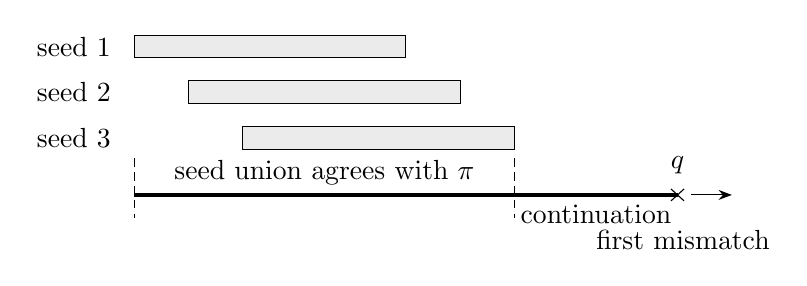
\begin{tikzpicture}[x=0.69cm,y=0.58cm,>=Stealth]
  \draw[fill=black!8] (1,2) rectangle (6,2.5);
  \draw[fill=black!8] (2,1) rectangle (7,1.5);
  \draw[fill=black!8] (3,0) rectangle (8,0.5);
  \node[anchor=east] at (0.75,2.25) {seed 1};
  \node[anchor=east] at (0.75,1.25) {seed 2};
  \node[anchor=east] at (0.75,0.25) {seed 3};
  \draw[densely dashed] (1,-0.2) -- (1,-1.5);
  \draw[densely dashed] (8,-0.2) -- (8,-1.5);
  \draw[very thick] (1,-1) -- (11,-1);
  \draw[->] (11.25,-1) -- (12,-1);
  \node[above] at (4.5,-1) {seed union agrees with $\pi$};
  \node[below] at (9.5,-1) {continuation};
  \draw (10.88,-1.13) -- (11.12,-0.87);
  \draw (10.88,-0.87) -- (11.12,-1.13);
  \node[above] at (11,-0.75) {$q$};
  \node[below] at (11.1,-1.55) {first mismatch};
\end{tikzpicture}
\caption{Different seed ends initiate the same first-mismatch test.
The overlapping seed union already agrees with the common repetition,
so no scan can stop inside a later seed.}
\label{fig:common-seeds}
\end{figure}

For an outer layer with full cut-offset set $\mathcal H_i$, a suffix
beginning at $k$ uses
\[
 \mathcal T=\{k-h:h\in\mathcal H_i\}.
\]
If the prefix chooses an actual cut $k=t+h_0$ with
$h_0\in\mathcal H_i$, the true origin belongs to this set regardless of
the suffix's independent role or tag.  Its diameter is
$\operatorname{diam}\mathcal H_i$.  Thus the end guard in
Lemma~\ref{lem:shared-anchor} establishes exact consumption before any
agreement of tags is used.  Likewise an aligned stencil $\mathcal P_i$
gives candidate origins $k+L_0-p'$; at a true cut $k=s+p$ these are
$t+p-p'$.  Their diameter is $\operatorname{diam}\mathcal P_i$.

\begin{lemma}[End selection after bounded decoding]\label{lem:decoded-end}
Let $e,k,[k,b),t,q$ be as in Lemma~\ref{lem:shared-anchor}, and let
$\mathcal T$ be any finite candidate set containing $t$, with no diameter
restriction.  Suppose its candidates are tested by bounded predicates
which do not use an anchor, all their inspection intervals lie inside
both the actual episode and the proposed suffix, and the true origin
passes its predicate.  If exactly one candidate passes, it is the true
origin.  Applying the exact end rule at that decoded origin, with its
search and seed data also present in both factors, forces the proposed
suffix to end at $q+B_{\rm tail}$ without any stability assumption.
\end{lemma}

\begin{proof}
The bounded predicates have the same values on their common letters,
so the passing true candidate cannot disappear in the proposed suffix.
Uniqueness therefore identifies it.  Apply
Lemma~\ref{lem:shared-anchor} with the singleton reference set $\{t\}$;
its equality condition is automatic.
\end{proof}

The last aligned stage will use Lemma~\ref{lem:decoded-end}.  Its current
witness is a bounded end-marker test independent of $q$, so decoding
precedes the end rule.  At the other stages one reference end rule is
applied first.  In either order, subsequent controls at translated
origins keep that same $q$ fixed.  They do not apply additional
first-mismatch searches.

\subsection{The finite margin interface}

The end guards require every bounded inspection to lie inside the true
episode, even when the suffix proposes a wrong origin or a wrong end.
This requirement can be met after all finite schedules have been chosen.
We state the margin calculation here; Proposition~\ref{prop:parameters}
will supply the complete inventory of inspections for the actual splits.

Take the union of the bounded inspection intervals under every allowed
cut, metadata choice, and candidate origin. Include the neighborhoods
needed to decide markers and the intervals swept out in
Lemma~\ref{lem:search-crossings}. Let $I_-\le0\le I_+$ bound the
inner-marker and trial data and all outer cuts relative to $t$, and let $E_-,E_+$ bound
the end-marker inspections and seed blocks relative to $z_\bullet(t)$.
These are finite bounds. The continuation to the selected first mismatch
is governed separately by the exact end rule; products ending there and
residues involving $q$ do not enlarge this bounded inventory.

Let $A$ bound the offsets from $s$ of the buffers before $t$.
Sufficient final margin inequalities are
\begin{equation}\label{eq:geometry-margins}
\begin{split}
 L_0+I_-&>A,\\
 o_\bullet+\min\{E_-,-d_\bullet\}&>I_+,\\
 B_{\rm tail}&>E_++d_\bullet,
 \qquad B_{\rm tail}\ge1.
\end{split}
\end{equation}
The first inequality puts all inner data after the early buffers.
The second puts the end controls and every possible anchor after the
inner data and the outer cuts included in that inventory. Since
$q\ge z_\bullet(t)-d_\bullet$, the last inequality puts every end
control strictly before even the earliest complete end
$z_\bullet(t)-d_\bullet+B_{\rm tail}$. Thus all bounded controls
are internal to every true complete episode.

Internal visibility does not by itself put data on the correct side of
a cut. Each split must also place its prefix computations before its cut
and its suffix computations after it. Any supplied left context must be
declared as finite metadata and verified by the prefix. The schedules in
Proposition~\ref{prop:parameters} will meet these reading-side conditions.

Every test argument must itself contain every position it is required
to inspect on its reading side. An unavailable candidate or translate
causes rejection; it is never omitted from a universal guard or uniqueness
test. Requested product intervals must likewise have available, correctly
ordered endpoints. This applies to a standalone suffix with false metadata
and to a proposed endpoint different from the true episode end. The margin
inequalities give availability for the true suffix; the rejection rule
ensures that every accepted suffix sees the same bounded control values
used in Lemmas~\ref{lem:shared-anchor} and~\ref{lem:decoded-end}.

The remaining obligation is to fix this finite inventory independently of
$L_0,o_\bullet,B_{\rm tail}$. Proposition~\ref{prop:parameters} does so
before choosing those three lengths in the order displayed above.

\section{Two outer splits and five residual witnesses}\label{sec:outer}

We first transmit the finite computation through prediction trials whose
boundaries are selected by markers. When a required boundary is absent,
a second split uses a long periodic interval to keep the prefix metadata
constant while varying the clock residue. Each construction defines a total
affine update before describing its successful cuts. The episodes where
neither construction supplies every input with a cut will have one of five
explicit witnesses.

The schedules in this section have fixed finite lengths and offsets for
the chosen monoid and alphabet. We state every separation and visibility
condition when it is used. Proposition~\ref{prop:parameters} constructs
all of them in one consistent order; until then they are the explicit
hypotheses of the two split constructions.

Use the episode start \(s\), sampling origin \(t=s+L_0\), anchor \(q\), and end
\(q+B_{\rm tail}\) from Definition~\ref{def:episodes}. Five later subbuffers
will lie between \(s\) and \(t\); the two splits of this section make their cuts
after \(t\). Write \(T_e=T_{s,q+B_{\rm tail}}\).

\subsection{The main schedule and the common end guard}

Fix the initial representation on \(V\), and put \(J=|V|^2\).
There is a finite collection of \emph{main trials}, indexed by \(\nu\),
with fixed predictions \(\Theta_\nu\in M^{J+1}\).
Let
\[
             \mathcal Z=\{(\nu,j):0\le j\le J+1\}
\]
label their endpoints and checkpoints. For \(\lambda\in\mathcal Z\), let
\(o_\lambda\) be its nominal offset from \(t\). Use an inner marker system
of separation \(d_\circ\), block length \(K_\circ>3d_\circ^2\), and radius
\(r_\circ\ge K_\circ\). Define
\begin{equation}\label{eq:main-boundaries}
\begin{split}
 z_\lambda(t)&=t+o_\lambda,\\
 u_\lambda(t)&=\text{first inner marker in }
 [z_\lambda(t)-H,z_\lambda(t)+H],
\end{split}
\end{equation}
with value \(\bot\) when the search is empty.
Let \(\mathcal A(t)\) mean that every \(u_\lambda(t)\) is present.
On \(\mathcal A(t)\), these are the actual ordered trial boundaries.
For trial \(\nu\), its actual endpoints are
\(B_\nu=u_{\nu,0}(t)\), \(C_\nu=u_{\nu,J+1}(t)\).
Its block \(j\) consists of cuts
\begin{equation}\label{eq:main-cuts}
                 k=t+c_{\nu,j}+a,\qquad 0\le a<R_1.
\end{equation}
The offsets place this entire block between boundaries \(j-1\) and \(j\).
All earlier-boundary searches, including their inspection neighborhoods, are
before the block; all later ones are after it. Trials are disjoint and ordered.

The second layer will use cuts
\begin{equation}\label{eq:periodic-cuts}
                     k=z_\lambda(t)+a,\qquad 0\le a<R_2.
\end{equation}
Let \(\mathcal H_1,\mathcal H_2\) be the respective full finite sets of cut
offsets from \(t\) in \eqref{eq:main-cuts} and \eqref{eq:periodic-cuts}.
Choose the end-stability radius with
\[
              \diam\mathcal H_1,\diam\mathcal H_2<w_E<d_\bullet,
 \qquad K_\bullet-w_E>d_\bullet^2.
\]

Every suffix test in outer layer \(r\in\{1,2\}\) uses the following guard,
independently of its tag. At its beginning \(k\), form \emph{all} origins
\[
                         k-h,\qquad h\in\mathcal H_r.
\]
Require their values of \(\eta\) to be equal, and require exact consumption
to the episode end obtained from one fixed reference origin in this set.
Let \(q\) be that reference anchor. All bounded guard data must be present
in the suffix argument.

If paired with an actual prefix cut, the true \(t\) belongs to this list.
Lemma~\ref{lem:shared-anchor} forces the reference anchor to be the true \(q\),
even if the proposed suffix initially extends beyond the first episode or
ends prematurely. Thus it consumes exactly the first episode. In particular
the clock integers supplied on the two sides,
\[
                            k-t,\qquad q-k,
\]
always have common total
\begin{equation}\label{eq:clock-total}
                              \ell=q-t.
\end{equation}
For availability, it suffices that \(\eta\) is stable under every shift of
magnitude at most \(w_E\), since this covers every reference origin relative
to the actual one.

\subsection{The main affine update}

Apply Lemma~\ref{lem:clock} to tags
\[
                 \alpha=(\nu,j,X,Y),\qquad X,Y\in V.
\]
Write the resulting clock as \(n_1,I^{(1)}_\alpha,J^{(1)}_\alpha,W_1\),
and let \(\mathcal G_1(\ell)\) be its graph of possible tag pairs.
Take \(R_1=n_1\).

Define \(F_{1,e}:V\to V\) for every episode, without referring to any split.
\begin{enumerate}[label=\textup{(\alph*)}]
\item If \(\mathcal G_1(\ell)\) is contained in the diagonal and
\(\mathcal A(t)\) holds, process letters normally except that each main trial
has the ideal deterministic shift of Lemma~\ref{lem:prediction} added at its end.
\item If \(\mathcal G_1(\ell)\) is contained in the diagonal and
\(\mathcal A(t)\) fails, use \(v\mapsto vT_e\).
\item If \(\mathcal G_1(\ell)\) has its unique off-diagonal edge
\(\alpha\to\beta\), use
\begin{equation}\label{eq:main-error}
                 F_{1,e}(v)=vT_e+Y(\beta)-X(\alpha)T_e.
\end{equation}
\end{enumerate}
These are exhaustive cases, including the empty graph in the diagonal case.
In every case \(F_{1,e}\) is deterministic affine with linear part \(T_e\).

Here and below a language with metadata is the finite union over
\emph{its own} metadata choices. Prefix and suffix unions are independent.
Let \(P_x^{(1)}\) require, for one tag \((\nu,j,X,Y)\):
\begin{enumerate}[label=\textup{(\roman*)}]
\item its length is one prescribed cut in \eqref{eq:main-cuts};
\(k-t\in I^{(1)}_\alpha\), and \(x=X\);
\item every boundary preceding the cut is present, including the boundaries
of all earlier trials and through boundary \(j-1\) of the current trial;
\item processing from \(x\) to \(B_\nu\), with ideal shifts on earlier trials,
arrives at the enumerated input \(x_j\) of this block;
\item the block's predicted transfer and all its preceding individual
interval conditions in Definition~\ref{def:eligibility} hold.
\end{enumerate}
All these data are before the cut, by placement.

Let \(Q_y^{(1)}\) use its own tag \((\nu,j,X,Y)\), the independent end guard,
the residue check \(q-k\in J^{(1)}_\alpha\), and \(y=Y\).
For each candidate
\begin{equation}\label{eq:main-role-origins}
                    k-c_{\nu,j}-a,\qquad 0\le a<R_1,
\end{equation}
perform the future-boundary searches for that role. Require every boundary
from \(j\) onward in the current trial, and every boundary in later trials,
to be present at the \emph{same word position} for all these candidates.
These searches are after \(k\) for every fixed role, whether the role is true
or false. Use their common positions to check the suffix-product condition
from boundary \(j\) to \(C_\nu\). From the block's enumerated output \(y_j\)
at \(C_\nu\), compute onward with ideal shifts in later trials and require
final result \(y\).

Define \(S_1\subseteq E\) by the following conditions on actual episode data:
\begin{equation}\label{eq:S1}
\begin{gathered}
 \eta(t)\text{ is stable within }w_E,\qquad
 \ell\notin W_1,\qquad \mathcal A(t),\\
 u_\lambda(t)\text{ is stable within }R_1\text{ for every }\lambda,\qquad
 \text{some main trial is perfectly predicted}.
\end{gathered}
\end{equation}
Stability means equality of the returned position or of the absent value for
every integer shift of either sign up to the indicated bound.

\begin{lemma}[Main split]\label{lem:main-split}
The languages \(P_x^{(1)},Q_y^{(1)}\) satisfy
Lemma~\ref{lem:split} on \(D=E\), with updates \(F_{1,e}\) and skipped class
\(E\setminus S_1\).
\end{lemma}

\begin{proof}
Take an arbitrary accepted prefix/suffix pair at a genuine episode boundary.
The end guard gives exact consumption and the common total \(\ell\).
If \(\mathcal G_1(\ell)\) is diagonal, the tags match. The actual \(t\)
then appears among \eqref{eq:main-role-origins}. The prefix establishes all
earlier boundaries and the suffix establishes all later boundaries, so
\(\mathcal A(t)\) holds. Their joint checks give an ideally eligible pair of
the actual current trial. Lemma~\ref{lem:prediction}, together with the ideal
computations before and after that trial, gives \(F_{1,e}(x)=y\).

If tags differ, the clock graph consists of that unique off-diagonal edge.
The input and output checks fix \(x=X(\alpha)\), \(y=Y(\beta)\), so
\eqref{eq:main-error} fits the transfer. The calculations performed under
possibly false roles introduce no competing input or output. These cases prove
soundness for every independent pair of witnesses.

For \(e\in S_1\) and input \(x\), select a perfect trial and its block for the
vector actually arriving there and its trial output. Choose the tag
\(X=x\), \(Y=F_{1,e}(x)\). Since \(\ell\notin W_1\), this diagonal tag pair
is available at some first residue. Its \(n_1\) consecutive cut choices realize
every such residue. Every role-origin differs from the true one by less than
\(R_1\), so future-boundary stability makes all suffix comparisons pass.
End stability makes the independent guard pass. All required data are present,
giving the desired split.
\end{proof}

The first split is sound on every episode, but its availability needs all
main boundaries and a perfect prediction. We next handle an episode with
a sufficiently long markerless boundary window. Its short-period run will
supply many cuts with identical prefix products and local contexts; only
the second clock residue changes.

\subsection{The periodic-window affine update}

To compute \(F_1\) on skipped sequences, use its homogeneous lift
\(\widehat F_{1,e}\) on
\[
                         U_0=V\oplus\mathbf F_2.
\]
Take a second clock with modulus \(n_2\), bad set \(W_2\), and tags
\begin{equation}\label{eq:second-tags}
 \alpha=(\lambda,X,Y,m,r,\xi),\qquad
 \begin{cases}
 \lambda\in\mathcal Z,\quad X,Y\in U_0,\\
 m\in M,\quad r\in\mathbb Z/n_1,\\
 \xi\in\Sigma^{2r_\circ}.
 \end{cases}
\end{equation}
These fields propose the boundary label, episode input/output, product
\(T_{s,k}\), residue \(k-t\bmod n_1\), and immediate left context of the cut.
There is no field for the cut index or \(n_2\).

Let \(\mathcal G_2(\ell)\) be its graph. On every episode define \(F_{2,e}\) to
be \(\widehat F_{1,e}\) in the diagonal case; in the unique off-diagonal case
\(\alpha\to\beta\), define
\begin{equation}\label{eq:second-error}
 F_{2,e}(v)=v\widehat F_{1,e}
       +Y(\beta)-X(\alpha)\widehat F_{1,e}.
\end{equation}
This is deterministic affine with linear part \(\widehat F_{1,e}\).

The prefix language \(P_x^{(2)}\) chooses its own tag and requires:
\begin{enumerate}[label=\textup{(\roman*)}]
\item a cut in \eqref{eq:periodic-cuts} for its label,
\(k-t\in I^{(2)}_\alpha\), and \(x=X\);
\item the proposed product \(m=T_{s,k}\), first-clock residue \(r\), and context
\(\xi\) are correct;
\item there is no inner marker in
\[
                           [z_\lambda(t)-H,k-r_\circ].
\]
\end{enumerate}
The marker decisions use only prefix data, since their radius is \(r_\circ\).

The suffix language \(Q_y^{(2)}\) uses its own tag, the second layer's independent
end guard, \(q-k\in J^{(2)}_\alpha\), and \(y=Y\).
Adjoin the proposed \(\xi\) immediately before its argument for the following
local test: require no inner marker in
\begin{equation}\label{eq:periodic-suffix-window}
                          [k-r_\circ,k+H+R_2].
\end{equation}
Exactly \(2r_\circ\) preceding letters suffice for the earliest radius
\(r_\circ\) decision. All other required letters must be in the suffix.

Use the proposed \(m\) and the actual suffix product to obtain a proposed
\(T_e\). Use \(r+(q-k)\bmod n_1\) as the proposed first-clock total.
Under the hypothesis \(\neg\mathcal A(t)\), these two data determine \(F_1\):
it is the linear action in the diagonal first-clock case and
\eqref{eq:main-error} in the off-diagonal case. Require
\[
                             y=X\widehat F_{1,e}
\]
as evaluated by precisely this rule. The suffix need not decode \(t\).

Put \(N_M=|M|!\), and require
\begin{equation}\label{eq:periodic-parameters}
\begin{gathered}
 R_2=n_2n_1N_Md_\circ,\qquad
 H-d_\circ>2r_\circ+|M|d_\circ+R_2,\\
 \text{every prime factor of }n_2\text{ exceeds }d_\circ,N_M,n_1.
\end{gathered}
\end{equation}
Within \(E\setminus S_1\), let \(S_2\) be the episodes with
\begin{equation}\label{eq:S2}
\begin{gathered}
 \eta(t)\text{ stable within }w_E,\qquad \ell\notin W_2,\\
 \text{for some }\lambda,\quad
 [z_\lambda(t)-H,z_\lambda(t)+H+2R_2]\text{ has no inner marker}.
\end{gathered}
\end{equation}

\begin{lemma}[Periodic-window split]\label{lem:periodic-split}
The second pair of languages satisfies Lemma~\ref{lem:split} on
\(D=E\setminus S_1\), with updates \(F_{2,e}\) and skipped class
\[
                        D_0=E\setminus(S_1\cup S_2).
\]
\end{lemma}

\begin{proof}
Again the independent guard gives exact consumption and total \(\ell\).
For matching tags, their product, residue and context are actual.
Since \(k=z_\lambda(t)+a\), \(0\le a<R_2\), the prefix absence interval and
\eqref{eq:periodic-suffix-window} cover the full actual search
\([z_\lambda(t)-H,z_\lambda(t)+H]\). Thus this boundary is absent and
\(\neg\mathcal A(t)\) is proved by the successful split.
The suffix has consequently evaluated \(\widehat F_{1,e}\) correctly.
In the diagonal second-clock case its output is \(F_{2,e}(x)\).
Mismatched tags fit the unique input/output pair in \eqref{eq:second-error}.
This proves soundness without assuming correctness of unmatched context.

For availability, let \(e\in S_2\), with the indicated center \(z\).
The marker property gives short-period \(K_\circ\)-blocks at all starts
from \(z-H+d_\circ\) through \(z+H-d_\circ\).
Lemma~\ref{lem:periodic-overlap} makes these one periodic run of some
period \(d<d_\circ\). The second inequality of
\eqref{eq:periodic-parameters} places all needed contexts and at least
\(|M|\) whole periods immediately before \(z\) within this run.

For any \(c\in M\), two of \(c^0,\ldots,c^{|M|}\) agree. Multiplying onward
gives an eventual period at most \(|M|\), starting before \(|M|\), and that
period divides \(N_M\). In particular
\[
                    c^{r+N_M}=c^r\qquad(r\ge|M|).
\]
Consider cuts
\begin{equation}\label{eq:special-cuts}
                k_a=z+a\,dN_Mn_1,\qquad 0\le a<n_2.
\end{equation}
They have \(0\le k_a-z<R_2\), identical \(2r_\circ\)-letter contexts,
and a fixed residue modulo \(n_1\). Take the period word in phase at \(z\),
with product \(c=T_{z,z+d}\), and put \(A=T_{s,z-|M|d}\). Then
\[
 T_{s,k_a}=Ac^{|M|+aN_Mn_1}=Ac^{|M|}.
\]
Thus the prefix-product field \(m\) is fixed. Although the suffix product
can vary with \(a\), it always satisfies \(mT_{k_a,q+B_{\rm tail}}=T_e\);
the recovered first-clock total is likewise always \(q-t\).
For input \(x\), one correct tag in \eqref{eq:second-tags}, with
\(X=x\) and \(Y=x\widehat F_{1,e}\), is therefore valid at all these cuts.
The prime-factor requirement gives
\(\gcd(dN_Mn_1,n_2)=1\). The cuts realize every residue modulo \(n_2\),
so one realizes this diagonal tag pair since \(\ell\notin W_2\).
Both absence tests lie in the markerless interval from \eqref{eq:S2}:
their rightmost endpoint is less than \(z+H+2R_2\), and their leftmost
positions are covered by the same margin. The stable end guard passes.
This gives a split for every input.
\end{proof}

We have two total updates and two availability sets. The remaining task
is to describe failure of both availability conditions using a fixed
number of predicates. These predicates will locate the true cut in the
aligned constructions of Section~\ref{sec:aligned}.

\subsection{The five witnesses}

We use the following predicates \(A_i(t,q)\) on episode data, and also at
formally translated sampling origins:
\begin{equation}\label{eq:witnesses}
\begin{array}{c@{\quad}p{0.80\linewidth}}
 i & \(A_i(t,q)\)\\ \hline
 0 & \(q-t\in W_1\), or \(\mathcal A(t)\) and no main trial is perfectly
 predicted at these boundaries;\\
 1 & some \(u_\lambda(t)\) changes under a shift of magnitude at most \(R_1\);\\
 2 & \(q-t\in W_2\);\\
 3 & some \([z_\lambda(t)-H,z_\lambda(t)+H]\) is markerless, but an inner
 marker lies among the next \(2R_2\) positions to its right;\\
 4 & \(\eta(t)\) changes under a shift of magnitude at most \(w_E\).
\end{array}
\end{equation}
In particular \(A_4\) does not use \(q\). Membership in a clock bad set always
uses the corresponding modulus.

At a translated origin, these are \emph{formal predicates on the given data},
with \(q\) fixed. They do not assert that the origin completes another episode,
and do not run another first-break scan. All marker decisions and products
they request will be internal to the available data.

\begin{lemma}[Residual coverage]\label{lem:witness-coverage}
Every episode of \(D_0\) satisfies at least one of \(A_0,\ldots,A_4\).
\end{lemma}

\begin{proof}
Suppose \(A_4\) fails. If \(\mathcal A(t)\) holds and both \(A_0,A_1\) fail,
all conditions of \(S_1\) hold. If \(\mathcal A(t)\) fails, choose a missing
boundary. Failure of \(A_2,A_3\) gives a good second-clock total and an empty
window extended by \(2R_2\) at that boundary, hence \(S_2\) unless the episode
was already in \(S_1\). Thus an episode in neither designation has a witness.
\end{proof}

\section{Aligned splits for the residual witnesses}\label{sec:aligned}

The two outer splits leave the task of computing $F_2$ on $D_0^*$.
Every episode in $D_0$ has one of the five witnesses from
Lemma~\ref{lem:witness-coverage}. We eliminate them in order. At stage $i$,
the current computation is a map $g_{i,e}:U_i\to U_i$, with
$g_{0,e}=F_{2,e}$ and $U_0=V\oplus\mathbf F_2$. We construct a new affine
update $g_{i+1,e}$ on a larger vector space. Two splits compute this new
update while removing the current witness; its linear part then recovers
$g_{i,e}$, by a basis encoding described below. The new update is the
same for both splits and is defined on every complete episode.

The witnesses serve to decode the cut position. A suffix tests every
candidate origin, excludes later witnesses there, and requires a unique
candidate with the current witness. After decoding, the first split uses
a perfectly predicted trial. On the remaining domain, a second split
uses a full decision tree to recover a prefix product from one of its
measurements. The secondary guard must exclude later witnesses on a
larger set of translates: this will ensure that the actual history has
no perfectly predicted trial. Proposition~\ref{prop:parameters} supplies
the finite schedules and ambiguity bounds used here.

\subsection{Stencils, domains, and the induction invariant}

For $i=0,\ldots,4$, place a nonempty finite stencil $\mathcal P_i$ of cut
offsets from $s$ in its own subbuffer. The buffers occur in the reverse
order $4,3,2,1,0$, after $s$ and before $t$, and the $i$-th ends at $a_i$.
Thus $a_{i+1}$ is before the entire stage-$i$ buffer whenever $i<4$.

\begin{figure}[htbp]
\centering
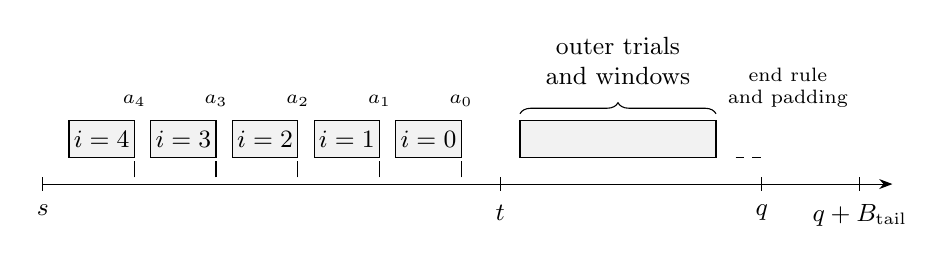
\begin{tikzpicture}[x=0.83cm,y=0.85cm,>=Stealth,font=\small]
 \draw[->] (0,0)--(13,0);
 \foreach \x/\label in {0/s,7/t,11/q,12.5/{q+B_{\rm tail}}}
   {\draw (\x,-.10)--(\x,.10);
    \node[below=4pt] at (\x,0) {$\label$};}
 \foreach \x/\i in {0.4/4,1.65/3,2.9/2,4.15/1,5.4/0}
   {\draw[fill=black!5] (\x,.4) rectangle ++(1,.55);
    \node at (\x+.5,.675) {$i=\i$};
    \draw (\x+1,.1)--(\x+1,.35);
    \node[above,font=\scriptsize] at (\x+1,1.02) {$a_{\i}$};}
 \draw[decorate,decoration={brace,amplitude=4pt}]
   (7.3,1.05)--(10.3,1.05);
 \node[above=7pt,align=center] at (8.8,1.05) {outer trials\\and windows};
 \draw[fill=black!5] (7.3,.4) rectangle (10.3,.95);
 \draw[dashed] (10.6,.4)--(11,.4);
 \node[above,font=\scriptsize,align=center] at (11.4,1.0)
       {end rule\\and padding};
\end{tikzpicture}
\caption{The aligned buffers occur in reverse stage order. For $i<4$, the
stage-$i$ buffer and the entire suffix beginning at $a_i$ lie after
$a_{i+1}$. Their data are therefore on the reading side of a suffix
starting at $a_{i+1}$. The drawing is schematic; the end-marker lag
and padding are chosen after every bounded inspection range.}\label{fig:reverse-buffers}
\end{figure}

Write
\begin{equation}\label{eq:gamma}
 \Delta_i=\mathcal P_i-\mathcal P_i,\qquad
 \Gamma_i=\sum_{j<i}(\Delta_j+\Delta_j),\qquad
 \Gamma_0=\{0\}.
\end{equation}
Every $\Delta_i,\Gamma_i$ contains zero, and
$\Gamma_{i+1}=\Gamma_i+\Delta_i+\Delta_i$.
For any finite set $\Gamma$, define
\[
 A_h^\Gamma(t,q)
 \quad\Longleftrightarrow\quad
 \text{there is }\gamma\in\Gamma\text{ with }A_h(t+\gamma,q).
\]
The anchor $q$ remains fixed. The entry domain $D_i\subseteq D_0$ has
the promise
\begin{equation}\label{eq:entry-promise}
                 \bigvee_{h\ge i}A_h^{\Gamma_i}(t,q).
\end{equation}
For $i=0$, this is Lemma~\ref{lem:witness-coverage}; the two full sets
defined below will give the induction step. Graph tests at stage $i$
concern $g_i$ on $D_i^*$, although every $g_{i,e}$ is defined on all
complete episodes.

The quantitative hypothesis is
\begin{equation}\label{eq:ambiguity-bound}
 \#\{(p,p')\in\mathcal P_i^2:p\ne p',\
                A_i^{\Gamma_i}(t+p-p',q)\}\le C_i.
\end{equation}
Every required kind of cut has more than $C_i$ copies in $\mathcal P_i$.
Also $h_i=\diam\mathcal P_i<w_E$ for $i<4$.
All witness controls at every candidate and every required translate
are after the cut and inside the true first episode. A suffix must
itself contain their full reading intervals to pass.

The reverse order of the buffers has a computational purpose. From
$a_{i+1}$, the whole stage-$i$ buffer and the suffix starting at $a_i$
are still unread. This lets a suffix formula for $g_i$ be incorporated
into a suffix formula for $g_{i+1}$, as shown next.



\subsection{Total tables and the new affine update}

The suffix beginning at $a_i$ does not know the product $T_{s,a_i}$ of
the omitted prefix. We therefore keep a table for every possible value
of that product. For fixed suffix letters and fixed $t,q$, the table is
a finite formula
\[
                 \Phi_i(m):U_i\longrightarrow U_i\qquad(m\in M)
\]
with
\begin{equation}\label{eq:table-property}
                      \Phi_i(T_{s,a_i})=g_{i,e}.
\end{equation}
It is defined for every $m$, including values that no prefix realizes.
It may use the indicated suffix, bounded marker data, $M$-products,
and fixed $t,q$. Evaluating this table is a finite calculation on one
episode; it is not a query to a graph language for a sequence of episodes.
We prove the existence of these tables inductively below.

To carry this table through another pair of splits, encode a payload
$v\in U_i$ and a work-register value $m\in M$ as a single basis vector.
Set
\[
                   U_{i+1}=\mathbf F_2^{\,U_i\times M}
\]
with basis $[v,m]$. A letter product $d\in M$ acts linearly by
$[v,m]\rho(d)=[v,md]$. At the end of the stage-$i$ buffer, replace the
remaining computation by the terminal linear map $H_i$ defined by
\begin{equation}\label{eq:late-map}
                    [v,m]H_i=[\Phi_i(m)(v),1_M].
\end{equation}
This is a linear extension from the displayed basis assignment; it
does not require $\Phi_i(m)$ to be linear on $U_i$. The unshifted
episode computation consists of $\rho(T_{s,a_i})$ followed by $H_i$.
No letter action follows $H_i$, which already represents the entire
remaining suffix. In particular,
\[
 [v,1_M]\rho(T_{s,a_i})H_i
   =[\Phi_i(T_{s,a_i})(v),1_M]
   =[g_{i,e}(v),1_M].
\]
Resetting the work register to $1_M$ makes the output suitable as the
input to the next episode. If $L_e=\rho(T_{s,a_i})H_i$, then for two
episodes $e,f$,
\[
                   [v,1_M]L_eL_f
                      =[g_{i,f}(g_{i,e}(v)),1_M].
\]
Thus products of these linear maps recover the composed $g_i$ update.
Our new affine update will have precisely $L_e$ as its linear part.

In the first part of the stage-$i$ buffer, take a full decision tree
with $b$ measurements along each path. A node has its own fixed
position $u$ and branches on $T_{s,u}\in M$, with a separate subtree
or leaf for every value. Ancestors precede descendants; all nodes
can be ordered topologically. The resulting leaf history depends
only on the letters, not on the input vector.

After all these measurements, place aligned prediction trials with
fixed endpoints, checkpoints, and blocks, using the representation
$\rho$. Put
\[
              J'=|U_{i+1}|^2,\qquad
              R=|M|^{J'+1},\qquad b>R.
\]
For every ordered list of $R$ distinct leaf histories, allocate a trial
whose predictions across those histories exhaust $M^{J'+1}$. Give
arbitrary predictions to its other histories, and include a spare
trial with arbitrary predictions. Every history has a prediction on
every trial, including histories that cannot occur on an actual prefix.
Only predictions depend on history; physical trial intervals do not.

Define $g_{i+1,e}$ by the unshifted computation above, adding the ideal
shift of Lemma~\ref{lem:prediction} at each stage-$i$ trial end, using
the actual leaf history. These are its only shifts. Before $a_i$,
any buffers of other stages contribute only their letter actions
$\rho$; their shifts and terminal maps are not applied there. The
shifts are constants determined by the episode, so they do not change
its linear part. This is why the two splits can compute $g_{i+1}$
and then recover $g_i$ by Lemma~\ref{lem:affine-recovery} and the
basis-state calculation above.

\begin{lemma}[Total suffix tables]\label{lem:total-tables}
The tables $\Phi_i$ exist for $0\le i\le4$.
Every $g_{i+1,e}$ just defined is deterministic affine, independent of
split success and domain restrictions. Its linear part $L_{i+1,e}$
satisfies
\begin{equation}\label{eq:basis-recovery}
                 [v,1_M]L_{i+1,e}=[g_{i,e}(v),1_M].
\end{equation}
The state spaces, tree sizes, and aligned trial counts depend only on
the preceding state sizes and $M$, not on the length or complexity of
a table formula.
\end{lemma}

\begin{proof}
For $i=0$, all main boundaries and trials are after $a_0$. Their
marker decisions and actual interval products are suffix data, and
both clock graphs depend on fixed $q-t$. Replace each required
$T_{s,z}$ by $mT_{a_0,z}$. The explicit rules of Section~\ref{sec:outer}
then compute $F_1$, its homogeneous lift, and $F_2$ for every $m$,
agreeing with $F_2$ at the actual prefix product. This gives $\Phi_0$.

For $i<4$, put $a=a_{i+1}$ and $b=a_i$. Every stage-$i$ measurement
and trial lies after $a$. A hypothetical product $m$ assigns
$mT_{a,u}$ to the measurement at $u$, selecting a leaf $h(m)$ in
the full tree. Let $C_\nu$ be the stage-$i$ trial ends, and compute
their ideal shifts $\beta_\nu(h(m))$ from that leaf's predictions
and the actual interval products. For every $x\in U_{i+1}$, set
\begin{equation}\label{eq:total-table-formula}
 \Phi_{i+1}(m)(x)=
 \left(x\rho(mT_{a,b})+
       \sum_\nu\beta_\nu(h(m))\rho(T_{C_\nu,b})\right)H_i.
\end{equation}
The first term transports the input to $b$; each summand transports
one trial shift from its insertion point to $b$. Each shift is added
once to the whole vector, and the terminal map is then applied
linearly. The result is affine in $x$.

Every basis value encountered by $H_i$ has a defined image because
$\Phi_i$ is total on $M$. Hence this formula is defined even for
an infeasible hypothetical $m$ or an arbitrary sum of basis vectors.
At $m=T_{s,a}$, it is exactly $g_{i+1,e}$. A hypothetical $m$ changes
the work evolution and selected history; it changes neither the
actual suffix interval products nor $t,q$. This proves the next
table property.

For fixed word data, the letter actions and terminal map are linear
and all inserted shifts are independent of the input. Removing the
shifts therefore gives the linear part $\rho(T_{s,a_i})H_i$, proving
\eqref{eq:basis-recovery}. All schedules and basis sets are finite
functions of the already specified state sizes and $M$; formula
complexity changes none of them.
\end{proof}

The update and its total suffix table are now fixed independently of
successful splits. We next define the primary and secondary full sets:
they determine where each split must be available, and never redefine
the update that both splits compute.

\subsection{Copies and full sets}

There are two sorts of stencil kinds.
\begin{enumerate}[label=\textup{(\roman*)}]
\item A \emph{trial kind} specifies an aligned trial, its block, and a leaf
history. Its copies lie inside that block.
\item A \emph{measurement kind} specifies a tree node and an input payload
\(x\in U_{i+1}\). Its copies lie before that node's measurement and after all
its ancestor measurements.
\end{enumerate}
Every offset is distinct, so recovering an offset recovers all its metadata.

Inside \(D_i\), define the primary full set \(\mathcal F_i\) by
\begin{equation}\label{eq:primary-full}
 \text{the true history has a perfect aligned trial},\qquad
             \neg A_h^{\Gamma_i+\Delta_i}(t,q)\quad(h>i).
\end{equation}
Put \(D_i'=D_i\setminus\mathcal F_i\).
Inside \(D_i'\), define the secondary full set \(\mathcal O_i\) by
\begin{equation}\label{eq:secondary-full}
             \neg A_h^{\Gamma_i+\Delta_i+\Delta_i}(t,q)\quad(h>i),
\end{equation}
and put \(D_{i+1}=D_i'\setminus\mathcal O_i\).
Every episode left in \(D_{i+1}\) has a later witness expanded by
\(\Gamma_{i+1}\), proving the next entry promise.
At \(i=4\), the secondary condition is empty, so \(D_5=\varnothing\).

Both splits at this stage transmit the \emph{same} \(g_{i+1,e}\) from
Lemma~\ref{lem:total-tables}. These full sets and residual restrictions do
not redefine it.

\subsection{An exact suffix decoder}

At a cut \(k=s+p\), the suffix lists all possibilities
\begin{equation}\label{eq:time-candidates}
                \tau_{p'}=k+L_0-p',\qquad p'\in\mathcal P_i.
\end{equation}
In a primary test, it requires absence of every later
\(A_h^{\Gamma_i}\) at every candidate. In a secondary test, this guard is
strengthened to absence of every later \(A_h^{\Gamma_i+\Delta_i}\).

For \(i<4\), do the \(q\)-free last-type checks first and require equality of
\(\eta\) across all candidates. Apply the exact end rule at one reference
candidate, as in Lemma~\ref{lem:shared-anchor}, and use its \(q\).
Then perform the other required later-type checks. Finally require a unique
\(p'\in\mathcal P_i\) such that \(A_i^{\Gamma_i}(\tau_{p'},q)\).

At \(i=4\), there is no later guard. Use the uniqueness test for
\(A_4^{\Gamma_4}\), which is \(q\)-free, and only after decoding apply the
exact end rule at the decoded origin. Both uniqueness tests range over all
of \(\mathcal P_i\). After decoding, require metadata of the appropriate
kind. Every bounded control is mandatory; an argument missing any required
window rejects.

\begin{lemma}[Time decoder]\label{lem:time-decoder}
Paired with a genuine stencil prefix in the promised domain \(D_i\),
a successful primary or secondary decoder returns the actual offset and
consumes exactly the first episode.
On its respective full set, all later guards pass at every stencil cut,
and at most \(C_i\) offsets fail uniqueness. Thus every required kind has
a successfully decoded copy.
\end{lemma}

\begin{proof}
For an actual cut \(p\), the candidate \(p'=p\) is the true \(t\);
the others are \(t+p-p'\).

For \(i<4\), the explicit equality/end guard and \(h_i<w_E\) give the true
\(q\), independently of any decoded metadata. The true complete episode
contains every bounded control, and the proposed suffix must contain those
same controls. Thus even a prematurely or excessively long proposed suffix
sees the same control values.
The later guard eliminates every later witness at the true origin.
Since \(\Gamma_i\subseteq\Gamma_i+\Delta_i\), this holds for either guard.
The entry promise forces the true current witness to pass. Uniqueness
therefore selects precisely the actual \(p\), and the shared anchor already
gives exact consumption.

For \(i=4\), the entry promise itself makes the true candidate pass the
\(q\)-free test. Internal visibility of all controls prevents any choice of
proposed length or two-sided extension from hiding it. Uniqueness first
recovers the true time; applying its end rule then forces exact consumption.
This argument uses no anchor to prove the uniqueness assertion.

For availability of the primary guard, a candidate differs from \(t\) by
an element of \(\Delta_i\), and \eqref{eq:primary-full} excludes every
corresponding later \(\Gamma_i\)-translate.
For the secondary guard, \eqref{eq:secondary-full} excludes the further
\(\Delta_i\)-expanded tests at every candidate.
When \(i<4\), both full conditions include absence of \(A_4(t)\), since all
expansion sets contain zero. This is stability for \emph{every} shift of
magnitude at most \(w_E\), so the equality/end guard is available.

The true candidate now passes at each stencil cut. If actual offset \(p\)
is ambiguous, some \(p'\ne p\) satisfies the condition counted in
\eqref{eq:ambiguity-bound}. Choosing one such \(p'\) for each ambiguous \(p\)
injects ambiguous offsets into the counted pairs. At most \(C_i\) offsets
are lost in the whole stencil, so more than \(C_i\) copies of each kind
leave a decodable copy of that kind.
\end{proof}

For the secondary split one further consequence is crucial. On \(D_i'\),
a successful guard includes absence of every later
\(A_h^{\Gamma_i+\Delta_i}(t,q)\) at the true candidate.
If the true history had a perfect trial, the episode would satisfy
\eqref{eq:primary-full}, contradicting membership in \(D_i'\).
Thus the true history has no perfect trial. The same conclusion holds on
the secondary full set by \eqref{eq:secondary-full}.
The extra expansion is necessary here: membership in \(D_i'\) alone
allows an episode with a perfect true-history trial whose primary full
condition fails because of a later witness. Without the strengthened
guard, the secondary test could discard the actual measurement value.

The decoder has separated time recovery from state recovery. Any accepted
pair now knows the actual copy and its metadata. On each full set, the
whole-stencil count guarantees a copy of every required kind. We use
these facts first for a trial and then for a tree measurement.

\subsection{Primary transmission}

The primary \(P_x\) requires a trial-copy length \(p\). It checks its metadata
history against the actual measurements, processes from \(x\) to the current
trial start, and verifies the enumerated arrival vector, predicted transfer,
and preceding individual interval products of that block.
The whole tree and all earlier trials are on its side.

The primary \(Q_y\) applies the primary time decoder. Using the decoded
history, trial and block, it checks the suffix-product condition and computes
from the enumerated trial-end output through all later stage trials and the
terminal map, requiring result \(y\). Whole other trial shifts are evaluated
by ideal eligibility. In particular, the late map is evaluated on its stored
basis work values; the suffix does not need to learn a separate actual prefix
product at the cut.

For an accepted pair, Lemma~\ref{lem:time-decoder} identifies exactly the same
metadata on both sides. The trial conditions give ideal eligibility, and
Lemma~\ref{lem:prediction} proves \(g_{i+1,e}(x)=y\).
For a primary full episode, choose a perfect true-history trial and its
eligible block for the actually arriving vector. There is a decodable copy
of that history/trial/block kind, giving a split for every input vector.

\subsection{Secondary transmission and bad histories}

\begin{lemma}[Bad histories]\label{lem:bad-histories}
Fix one episode and the actual product tuples on all its aligned trial
intervals. Fewer than \(R\) leaf histories have no perfectly predicted trial,
including infeasible histories. Along the true path, fewer than \(R\) nodes
have a wrong proposed measurement value whose suffix continuation yields
such a history.
\end{lemma}

\begin{proof}
Let \(\mathcal B\) be the set of \emph{all} leaf histories whose prediction
differs from the actual tuple on every trial. If \(R\) distinct leaves
belonged to \(\mathcal B\), their allocated common trial would assign all
\(R\) possible tuples across those leaves. One assignment equals that trial's
actual tuple, a contradiction. Thus \(|\mathcal B|<R\).

At a true-path node with measurement \(u\), a wrong proposed value \(d\)
chooses a different branch. Continue at any later measurement \(u'\) using
\(dT_{u,u'}\). This selects a well-defined leaf in the off-path subtree,
whether or not the whole history is feasible.
Departures at two different nodes of the true path lie in disjoint subtrees,
so their leaves differ. Selecting one wrong surviving value at each ambiguous
node injects those nodes into \(\mathcal B\), proving the bound.
\end{proof}

The secondary \(P_x\) requires a measurement-copy length, verifies that its
node lies on the true path by checking ancestor measurements, and requires
payload \(x\).

The secondary \(Q_y\) applies the strengthened time decoder and obtains the
node, its ancestor-path metadata, and payload. At the node's measurement
position \(u\), try every \(d\in M\). Follow its branch and every later branch
using \(dT_{u,u'}\), and retain exactly the values whose resulting history
has no perfectly predicted trial. Require a unique retained value.

On an accepted pair in \(D_i'\), the true history has no perfect trial by
the strengthened-guard consequence above. Its actual value \(T_{s,u}\)
therefore survives, and uniqueness identifies it.
This datum suffices to compute the full update on every payload, not only on
a single basis vector. Indeed, if
\[
                        x=\sum_{v,m}c_{v,m}[v,m],
\]
then before \(u\) there have been no shifts in \(g_{i+1,e}\), and the vector
there is
\begin{equation}\label{eq:secondary-payload}
                x\rho(T_{s,u})
                   =\sum_{v,m}c_{v,m}[v,mT_{s,u}].
\end{equation}
The suffix knows all subsequent letters and trials, and all their ideal
shifts from the recovered history. It simulates to \(a_i\), applies the
total terminal map termwise, and requires result \(y\).
Each affine shift is added once to this entire vector, after the linear
work action; it is not added separately to each basis summand. The final
map \(H_i\) is applied once by linearity, and no letter action follows it.
No inverse in \(M\) is used.

For availability on a secondary full episode, the true history survives.
Lemma~\ref{lem:bad-histories} and \(b>R\) provide a true-path node at which no
wrong value survives. For any input payload, a decodable copy of its node
and payload kind exists. All continuation checks are after that cut, so this
copy gives an accepted split.

\subsection{The recursive conclusion}

\begin{lemma}[Aligned stage]\label{lem:aligned-stage}
Assume the entry promise, the table and placement properties, and
\eqref{eq:ambiguity-bound}, with more than \(C_i\) copies per kind.
Exact graph tests for \(g_{i+1}\) on \(D_{i+1}^*\) yield graph tests for
\(g_i\) on \(D_i^*\) by two uses of Lemma~\ref{lem:split} and finite Boolean
operations. All required hypotheses hold at the next residual stage, and
\(D_5=\varnothing\).
\end{lemma}

\begin{proof}
The secondary split first gives graph tests for \(g_{i+1}\) on \((D_i')^*\).
The primary split uses these as skips and gives its graph tests on \(D_i^*\).
Both splits act on \(U_{i+1}\) with the same deterministic affine update
\(g_{i+1}\). By
Lemma~\ref{lem:affine-recovery} these determine the product of its episode
linear parts. Equation~\eqref{eq:basis-recovery} shows that starting from
\([v,1_M]\), this product ends at \([g_{i,w}(v),1_M]\).
Thus finite basis-state queries recover the required graph tests for \(g_i\).

The domain promise and empty terminal domain follow from the definitions of
the full sets, and the next total table follows from
Lemma~\ref{lem:total-tables}. Starting with identity graph tests on the empty
\(D_5\) domain, the five stages consequently produce graph tests for
\(g_0=F_2\) on \(D_0^*\).
\end{proof}


\section{Choosing the parameters}\label{sec:parameters}

The preceding splits require two properties of their finite schedules.
For each aligned stage, the number of ambiguous cut offsets must be
smaller than the number of copies of every cut kind. At the same time,
every prefix and suffix test must see its prescribed data, including
the bounded controls at all false candidate origins. We now choose
the schedules so that both properties hold.

The number of cut kinds and the positions of their copies play different
roles. Enlarging the stage-0 roster creates more main trials and tags,
but the clock obstruction bound grows only logarithmically with the
tag count. This lets us fix the number of copies first. Their integer
positions remain free until the clocks and marker windows have fixed
the required main-trial width. The order of choices below makes this
separation explicit.

Throughout this section \(q\) is the anchor of the true episode.
Evaluating \(A_j(t+\delta,q)\) keeps that anchor fixed; it never
starts a new episode-end search at \(t+\delta\). This convention is
needed both for the clock estimates and for finite final padding.

\begin{proposition}\label{prop:parameters}
For every fixed nonempty finite alphabet, finite monoid \(M\), and
finite representation space \(V\), all parameters in the two outer
splits and the five aligned stages can be chosen to satisfy their
stated hypotheses. More precisely, the stencils are nonempty, have
more than \(C_i\) copies of each required kind, and satisfy
\[
 \#\{(p,p')\in\mathcal P_i^2:p\ne p',\
       A_i^{\Gamma_i}(t+p-p',q)\}\le C_i
       \qquad(0\le i\le4)
\]
on every complete episode. Write \(N_i=|\mathcal P_i|\).
In order, these bounds concern first-clock or prediction failure,
inner-search instability, second-clock failure, a right-margin marker,
and end-search instability. The constants can be taken to be
\begin{align}
 C_0&=K+c_{\rm cl}\log(2m_1),\label{eq:parameter-c0}\\
 C_1&=10|\mathcal Z|N_0^4(2R_1+3),\label{eq:parameter-c1}\\
 C_2&=N_0^4N_1^4c_{\rm cl}\log(2m_2),\label{eq:parameter-c2}\\
 C_3&=10|\mathcal Z|(2R_2+3)\prod_{j<3}N_j^4,
       \label{eq:parameter-c3}\\
 C_4&=10(2w_E+3)\prod_{j<4}N_j^4.
       \label{eq:parameter-c4}
\end{align}
Here \(K=|M|^{|V|^2+1}\), \(m_1,m_2\) are the respective full tag
alphabet sizes, and \(c_{\rm cl}\) is the absolute constant of
Lemma~\ref{lem:clock}; logarithms are natural. Also,
\(\operatorname{diam}\mathcal P_i<w_E\) for \(i<4\).
All measurements, trials, and inspections have the chronological and
reading-side access required in Lemmas~\ref{lem:main-split},
\ref{lem:periodic-split}, and~\ref{lem:aligned-stage}. Every bounded
control, including every control at a false candidate origin, lies
inside the true first episode. The same choices satisfy the end
margins of Section~\ref{sec:geometry}.
\end{proposition}

\begin{proof}
Write \(\kappa_i\) for the number of cut kinds at stage \(i\), and
use \(\mu_i\) copies of each kind, so that
\(N_i=\kappa_i\mu_i\). We will choose the finite objects in the
following order and verify each estimate as its inputs become fixed.
\begin{enumerate}
\item Fix the spaces \(U_i\), full trees, aligned trial identities,
      and prediction assignments. These determine the numbers
      \(\kappa_i\) before any clock or position is chosen.
\item Choose the stage-0 copy count \(\mu_0\) and its abstract roster.
      This fixes the main-trial identities and predictions, the first
      tag count \(m_1\), and \(\mathcal Z\). Choose the first clock
      and \(R_1\), retaining its prescribed roster residues but
      leaving the integer stage-0 positions open.
\item Choose the stage-1 count and numerical stencil. Then choose
      the inner marker separation \(d_\circ\), block length
      \(K_\circ\), and inspection radius \(r_\circ\).
\item Fix the second tag alphabet, choose the stage-2 count, and
      construct the second clock and numerical stencil. Then fix
      the periodic-window width \(R_2\).
\item Choose the stage-3 count and numerical stencil. Then choose
      the inner search halfwidth \(H\) and a common main-trial
      template large enough for all the prescribed inspections.
\item Place the stage-0 stencil with its reserved residues and with
      differences separated by more than this template length.
      Place the main trials; this determines the outer cut sets.
\item Choose the end-stability radius \(w_E\), then the stage-4
      count and numerical stencil, and finally the end marker
      parameters \(d_\bullet,K_\bullet,r_\bullet\).
\item Translate the aligned arrangements into reverse stage order.
      Choose \(L_0\), then \(o_\bullet\), then \(B_{\rm tail}\)
      to put every bounded inspection inside the true episode.
\end{enumerate}

At steps 3--5 the stage-0 positions, and hence the numerical sets
\(\Gamma_1,\Gamma_2,\Gamma_3\), are not yet fixed. Their cardinalities are already
bounded in terms of the chosen roster sizes. The clock and marker
estimates are uniform in the translated origin and in the nominal
search centers, so these cardinality bounds suffice until the actual
positions are selected. The only copy count that enters its own
obstruction bound is \(\mu_0\); its logarithmic dependence will be
resolved explicitly below.

\subsection*{Finite kinds before numerical parameters}
Put \(m=|M|\). The sets
\[
 U_0=V\oplus\mathbf F_2,
 \qquad U_{i+1}=\mathbf F_2^{\,U_i\times M}\quad(0\le i\le4)
\]
are fixed now; in particular
\( |U_{i+1}|=2^{m|U_i|}\).
At stage \(i\), set
\[
 J_i^{\rm al}=|U_{i+1}|^2,
 \qquad K_i^{\rm al}=m^{J_i^{\rm al}+1},
 \qquad b_i=K_i^{\rm al}+1.
\]
Use the full rooted \(m\)-ary tree with \(b_i\) measurements along each
root-to-leaf path. It has
\[
 e_i=\sum_{j=0}^{b_i-1}m^j
 \quad\hbox{measurement nodes},\qquad
 \ell_i=m^{b_i}\quad\hbox{leaves}.
\]
These formulas also apply when \(m=1\). For integers \(a,r\ge0\),
write \((a)_r=a(a-1)\cdots(a-r+1)\) when \(r\le a\), and
\((a)_r=0\) when \(r>a\). Allocate one aligned trial for each ordered
list of \(K_i^{\rm al}\) distinct leaves, and one spare trial. There
are \(\tau_i=1+(\ell_i)_{K_i^{\rm al}}\) trials.
On a listed trial, assign the \(K_i^{\rm al}\) possible product tuples
bijectively to its listed leaves; assign arbitrary tuples to all
other leaves. The spare trial has arbitrary predictions. Thus every
history, including every infeasible history, has a prediction on every
trial, as required in Lemmas~\ref{lem:total-tables}
and~\ref{lem:bad-histories}.

There is one measurement kind for each node and payload in
\(U_{i+1}\), and one trial kind for each trial, block, and leaf. Hence
the number of kinds introduced above is
\begin{equation}\label{eq:parameter-kinds}
 \kappa_i=e_i|U_{i+1}|+
              \tau_iJ_i^{\rm al}\ell_i.
\end{equation}
None of these sets or counts involves a clock, a marker radius, a
main-trial identity, or a numerical position. In the terminal map
\([v,a]\mapsto[\Phi_i(a)(v),1_M]\), the argument set \(U_i\times M\)
and the output basis set are already fixed. A later, more complicated
formula for the total table \(\Phi_i\) therefore does not introduce
new kinds or enlarge the spaces. The formulas in
Lemma~\ref{lem:total-tables} evaluate every hypothetical product; they
do not add a prefix-feasibility field to a kind.

We fix an ordering of these kinds and their eventual copies compatible
with the following finite event order. First order the tree nodes
topologically, so that each ancestor precedes its descendants.
Place all copies for a node before that node's measurement, and place
that measurement before the copies for every subsequent node.
After all measurements, place the aligned trials in order, with their
blocks in order and all copies for a block between its neighboring
boundaries. Checkpoints and trial starts and ends are interposed in
the indicated order. The extra ordering between unrelated nodes is
harmless. In particular, every measurement copy sees its ancestor
measurements before the cut and its own and descendant measurements
after the cut; every aligned trial follows the entire tree.

\subsection*{Separated differences with prescribed residues}
We shall repeatedly use the following elementary construction.
Given a finite ordered roster, a modulus \(n\ge1\), an assigned residue
for every roster slot, and an integer \(S\ge1\), there are increasing
integer positions for the slots with those residues such that all
nonzero ordered differences are distinct and are separated from each
other and from zero by more than \(S\).  Any fixed finite number of
interposed events can also be accommodated in each prescribed gap.

Here is a direct induction.  Suppose the already chosen positions are
\(x_1<\cdots<x_a\), with all their positive differences separated by
more than \(S\), and each positive difference greater than \(S\).
Their largest positive difference is \(D=x_a-x_1\), taking \(D=0\)
when \(a=1\).  Choose \(x_{a+1}\) in its prescribed residue class so
large that
\[
 x_{a+1}-x_a>D+S,
\]
and also so that the gap has room for every event to be inserted
there.  The new positive differences all exceed \(D+S\).  The
difference of two of them is an old point gap, and is greater than
\(S\).  They are consequently separated from one another and from all
old differences.  Their negatives have the same property, and the
positive and negative differences are separated through zero.
The first gap can be chosen greater than \(S\), initiating the
induction.  Arbitrarily large representatives of every residue class
exist, so no residue restricts this choice.  Events are then placed
at distinct integer positions inside the reserved gaps.  Extra room
before the first and after the last cut accommodates any exterior
trial boundaries.

We shall choose each stencil together with its interposed events in
this way.  Denote its diameter by \(h_i\).  A subsequent translation
of the entire stage changes none of its differences or internal
chronology.  In particular, if before translation its residues are
\(v_p\), then afterwards they are \(v_p+c\) for one constant \(c\);
all differences \(v_{p'}-v_p\) used by the clock remain unchanged.

For every such stencil,
\( |\Delta_i|\le N_i^2\) and
\( |\Delta_i+\Delta_i|\le N_i^4\).
The cardinality of a sumset is at most the product of the
cardinalities of its summands, whence
\begin{equation}\label{eq:parameter-gamma-size}
 |\Gamma_i|\le\prod_{j<i}N_j^4,
 \qquad
 \Gamma_i\subseteq
 \left[-2\sum_{j<i}h_j,\,2\sum_{j<i}h_j\right].
\end{equation}
All these sets contain zero.  The second formula is a bound on the
absolute values of their elements, not a bound by the same number on
their diameters.

\subsection*{Stage 0: the number of copies and the first clock}
Put \(J=|V|^2\) and \(K=m^{J+1}\).  Initially regard \(\mathcal P_0\)
as an indexed roster, without numerical positions.  With
\(N_0=\kappa_0\mu_0\), it has \(Q=N_0(N_0-1)\) ordered pairs of
distinct slots.  For every ordered list of \(K\) distinct such pairs,
allocate a group of \(K\) main trials, whose predictions exhaust
\(M^{J+1}\).  Include one spare main trial.  Thus the number of main
trials is
\[
 T_1=1+K(Q)_K\le1+KN_0^{2K}.
\]
The full first tag alphabet consists of trial, block, and two vectors
in \(V\).  Consequently
\begin{equation}\label{eq:parameter-main-tags}
 m_1=J|V|^2T_1=J^2T_1
       \le J^2(1+KN_0^{2K}),
 \qquad |\mathcal Z|=(J+2)T_1.
\end{equation}
No position or clock modulus occurs in this count.

For completeness, the simultaneous requirement
\(\mu_0>K+c_{\rm cl}\log(2m_1)\) has the following explicit solution.
Define constants, independently of \(\mu_0\), by
\[
 A=K+c_{\rm cl}\log\bigl(2J^2(1+K\kappa_0^{2K})\bigr),
 \qquad B=2c_{\rm cl}K.
\]
Choose an integer
\begin{equation}\label{eq:parameter-copy0}
 \mu_0>\max\{1,2A,4B^2\}.
\end{equation}
For \(\mu_0\ge1\), Equation~\eqref{eq:parameter-main-tags} gives
\[
 K+c_{\rm cl}\log(2m_1)
 \le A+B\log\mu_0
 \le A+B\sqrt{\mu_0}<\mu_0.
\]
We used \(\log x\le\sqrt x\) for \(x\ge1\), which follows, for
example, by minimizing \(\sqrt x-\log x\); its minimum is
\(2-\log4>0\).  This proves the desired strict inequality without a
fixed-point assumption about the clock size.

Fix this roster, tag alphabet, prediction schedule, and
\(\mathcal Z\).  Apply Lemma~\ref{lem:clock} with this roster and
prime threshold \(1\), obtaining \(n_1,W_1\) and roster residues.
Set \(R_1=n_1\).  Reserve the prescribed residues for the stage-0
positions.  Their actual integer values will be chosen only after
the common main-trial template length is known.

\subsection*{Stage 1 and the inner marker system}
Choose
\(\mu_1=\lfloor C_1\rfloor+1\), with \(C_1\) as in
Equation~\eqref{eq:parameter-c1}; all its inputs are now fixed.  Construct
the stage-1 stencil and event order with separated differences, using
modulus \(1\), and record \(h_1\).  Choose integers
\begin{equation}\label{eq:parameter-inner-marker}
 d_\circ>10(2h_1+2R_1+5),
 \qquad K_\circ>3d_\circ^2,
\end{equation}
and obtain the inner marker rule from Lemma~\ref{lem:markers}, with
an integer inspection radius \(r_\circ\ge K_\circ\).

To prove the stage-1 count, fix \(\gamma\in\Gamma_1\) and a boundary
label \(\lambda\).  As the nonzero difference \(\delta=p-p'\)
varies, the center
\(t+\gamma+o_\lambda+\delta\) lies in an interval of diameter
\(2h_1\).  If the first-marker search changes under some shift of
absolute value at most \(R_1\), a marker lies within \(R_1\) of one
of the two original search endpoints.  For either endpoint, the
swept interval has diameter \(2h_1+2R_1<d_\circ\), so contains at
most one marker.  Such a marker accounts for at most \(2R_1+1\)
integer values of \(\delta\).  This is also the endpoint-crossing
estimate of Lemma~\ref{lem:search-crossings}; it does not depend on
the as yet unchosen halfwidth \(H\).  Distinct nonzero differences
identify distinct ordered pairs.  Summing over the two endpoints,
\(\gamma\), and \(\lambda\) gives
\[
 \#\{(p,p'):p\ne p',\ A_1^{\Gamma_1}(t+p-p',q)\}
 \le2(2R_1+1)|\mathcal Z|N_0^4<C_1.
\]
The choice of nominal boundary positions will not affect this count.

\subsection*{Stage 2 and the second clock}
The full second tag alphabet is now fixed.  Its fields have sizes
\( |\mathcal Z|\), \(|U_0|\), \(|U_0|\), \(m\), \(n_1\), and
\(|\Sigma|^{2r_\circ}\), respectively.  We take the whole Cartesian
product, including tags that no particular word realizes.  Therefore
\begin{equation}\label{eq:parameter-second-tags}
 m_2=|\mathcal Z|\,|U_0|^2m n_1|\Sigma|^{2r_\circ}.
\end{equation}
Neither the second modulus nor the cut index in a periodic window is
a field.  Choose \(\mu_2=\lfloor C_2\rfloor+1\), and apply
Lemma~\ref{lem:clock} to the resulting stage-2 roster, with threshold
\(\max\{n_1,N_M,d_\circ\}\), where \(N_M=m!\).  This gives
\(n_2,W_2\) and the stage-2 roster residues.  Construct its numerical
stencil with these residues and separated differences, and record
\(h_2\).  Set
\begin{equation}\label{eq:parameter-r2}
 R_2=n_2n_1N_Md_\circ.
\end{equation}
For a fixed \(\gamma\in\Gamma_2\), the stage-2 predicate on an
ordered pair is exactly
\[
 q-t-\gamma+p'-p\in W_2.
\]
Here \(q-t-\gamma\) is fixed while the pair varies.  The roster bound
therefore gives at most \(c_{\rm cl}\log(2m_2)\) pairs for this
\(\gamma\).  Equation~\eqref{eq:parameter-gamma-size} proves the bound
\(C_2\). The clock estimate is uniform in the translate \(q-t-\gamma\);
only \(|\Gamma_2|\), not its eventual numerical values, enters this bound.

Every prime factor of \(n_2\) exceeds \(n_1,N_M,d_\circ\).
For each \(1\le d<d_\circ\), it follows that
\[
 \gcd(n_2,dN_Mn_1)=1.
\]
Thus the cuts with displacements
\(a dN_Mn_1\), \(0\le a<n_2\), run through every second-clock
residue.  Each displacement is less than \(R_2\), as required by
Lemma~\ref{lem:periodic-split}.

\subsection*{Stage 3 and the inner search halfwidth}
Choose \(\mu_3=\lfloor C_3\rfloor+1\), construct the stage-3 stencil
with separated differences, and record \(h_3\).  Choose an integer
\begin{equation}\label{eq:parameter-h}
 H>10\bigl(h_3+R_2+r_\circ+d_\circ(1+m)+1\bigr).
\end{equation}
Fix \(\gamma\in\Gamma_3\) and \(\lambda\). The relevant centers lie in an
interval of diameter \(2h_3\). Apply Lemma~\ref{lem:search-crossings}(ii)
with \(D=2h_3\), \(L=H\), and \(h=2R_2\).
Equation~\eqref{eq:parameter-h} gives \(D<2L+2\).
At most \(2R_2\) centers have the required empty search and right-margin
marker. Distinct ordered differences identify distinct ordered pairs,
and a union bound gives
\[
 \#\{(p,p'):p\ne p',\ A_3^{\Gamma_3}(t+p-p',q)\}
 \le2R_2|\mathcal Z|\prod_{j<3}N_j^4<C_3.
\]
This argument is independent of the nominal positions of the
boundaries.  Equation~\eqref{eq:parameter-h} also implies the separate
periodic-window requirement
\begin{equation}\label{eq:parameter-periodic-margin}
 H-d_\circ>2r_\circ+m d_\circ+R_2.
\end{equation}
Indeed, subtracting the right side from the left and using
Equation~\eqref{eq:parameter-h} leaves a positive quantity.  Together
with \(K_\circ>3d_\circ^2\), this supplies both the overlapping
short-period blocks and all the context and stabilized-power
margins used in Lemma~\ref{lem:periodic-split}.

At this point the first three numerical stencils, both clocks, the inner
marker radius, and the periodic-window width have all been fixed. The
only postponed early choice is the numerical stage-0 stencil. We can
now place it with gaps exceeding the complete main-trial template while
preserving the first-clock residues chosen earlier.

\subsection*{The main template and the postponed stage-0 positions}
Choose an even integer
\[
 G>10(H+r_\circ+R_1+R_2+1),
 \qquad T=(J+3)G.
\]
The common template is the interval of length \(T\).  Boundary
\(i\), \(0\le i\le J+1\), has center \((i+1)G\) relative to its
start; block \(j\), \(1\le j\le J\), begins at
\(jG+G/2\) and has the \(R_1\) consecutive cut positions prescribed
in Section~\ref{sec:outer}.  All boundary inspection windows, and
all periodic-window cuts and their inspection neighborhoods, fit
strictly inside the template.  For a block cut, its preceding
boundary's entire inspection window lies to the left, and the next
boundary's entire inspection window lies to the right.
The same holds for the future searches under every origin
\(k-c_{\nu,j}-a\), \(0\le a<R_1\): relative to \(k\) the nearest
future center is \(G/2-a\), which exceeds \(H+r_\circ\).
The nearest preceding center for the actual prefix is
\(-G/2-a\), whose whole inspection window precedes the cut.
Earlier and later trial windows have still larger separations.
The periodic suffix's absence test uses starts from
\(k-r_\circ\) onward, so a marker inspection needs no letter earlier
than \(k-2r_\circ\).  This is exactly the context length included
in its tag.

We may now choose the numerical positions of the stage-0 roster,
with its previously prescribed first-clock residues.  Use the
separated-difference induction with spacing \(S=T\), reserving all
aligned events in their required order.  Record \(h_0\).
For each allocated group, let
\(\delta_a=p_a-p'_a\), \(1\le a\le K\), be the differences of its
listed pairs.  Give its trial \(a\) the template start
\begin{equation}\label{eq:parameter-translated-template}
 b_{\rm group}-\delta_a
\end{equation}
relative to \(t\), retaining the prediction already assigned to
that abstract trial.  The differences are distinct and separated by
more than \(T\), so the templates within a group are disjoint.
Bases for distinct groups can be chosen explicitly.  Put the spare
trial at offset \(T\), enumerate the groups by \(g=1,\ldots,(Q)_K\),
and take
\[
 b_g=T+g(2h_0+2T)+h_0.
\]
Every group lies between offsets
\(T+g(2h_0+2T)\) and
\(T+g(2h_0+2T)+2h_0+T\).  These intervals are positive, mutually
separated, and disjoint from the spare template.  Sort all trials by
physical position for the processing rules.  Sorting changes neither
their identities nor their assigned predictions.  It now determines
all \(o_\lambda,c_{\nu,j},\mathcal H_1,\mathcal H_2\).

It remains to justify \(C_0\).  Its first-clock part contributes at
most \(c_{\rm cl}\log(2m_1)\), since
\[
 q-(t+p-p')=q-t+p'-p
\]
and the first-clock roster differences have been preserved.
Suppose that the prediction-failure part held for \(K\) distinct
ordered pairs.  Take their ordered list and its allocated group.
At origin \(t+\delta_a\), the indicated trial has physical template
start
\[
 (t+\delta_a)+(b_{\rm group}-\delta_a)=t+b_{\rm group}.
\]
All these \(K\) trials therefore have identical physical boundary
search centers.  The predicate under consideration includes
\(\mathcal A(t+\delta_a)\), so all their boundaries exist.
Locality and translation equivariance of the marker rule give the
same actual boundary positions, hence the same actual tuple of
\(J+1\) interval products, for all \(K\) trials.  Their predictions
exhaust all possible tuples; one must be perfect.  This contradicts
the assumed absence of any perfectly predicted main trial at its
origin.  There are thus at most \(K-1\) prediction-failure pairs,
and the total is strictly less than \(C_0\).  If the roster has fewer
than \(K\) ordered pairs, that last assertion already follows from
its size.  The internal visibility needed for this argument, including
all translated templates, is established below.

\subsection*{Stage 4 and the end marker system}
Choose an integer
\begin{equation}\label{eq:parameter-we}
 w_E>1+\max\left\{
 \operatorname{diam}\mathcal H_1,
 \operatorname{diam}\mathcal H_2,
 2(h_0+h_1+h_2+h_3)\right\}.
\end{equation}
In particular \(h_i<w_E\) for \(i<4\).  Choose
\(\mu_4=\lfloor C_4\rfloor+1\), construct its stencil with separated
differences, and record \(h_4\).  Choose integers
\begin{equation}\label{eq:parameter-end-marker}
 d_\bullet>10(2h_4+2w_E+5),
 \qquad K_\bullet>3d_\bullet^2,
\end{equation}
and obtain its marker rule and radius \(r_\bullet\ge K_\bullet\).
These choices imply
\[
 w_E<d_\bullet,
 \qquad K_\bullet-w_E>d_\bullet^2,
\]
so Lemma~\ref{lem:shared-anchor} applies to each required set of
unexpanded candidate origins.
For fixed \(\gamma\in\Gamma_4\), apply the same endpoint argument as
at stage 1, with center range of diameter \(2h_4\), stability radius
\(w_E\), and marker separation \(d_\bullet\).  Each endpoint sweep
has diameter \(2h_4+2w_E<d_\bullet\), and the number of bad
nonzero differences is at most \(2(2w_E+1)\).  Hence
\[
 \#\{(p,p'):p\ne p',\ A_4^{\Gamma_4}(t+p-p',q)\}
 \le2(2w_E+1)\prod_{j<4}N_j^4<C_4.
\]
This count is independent of the end search's eventual lag.

All five ambiguity bounds are now proved, and each stencil has more
copies per kind than its bound. It remains to put the finite arrangements
inside words. This last step must cover every false-origin inspection,
not only the windows used by a correctly chosen split.

\subsection*{Final placement and visibility under every hypothesis}
Translate the five complete aligned arrangements, including all
interposed events, into disjoint integer intervals strictly after
\(s\), in order \(4,3,2,1,0\).  End stage \(i\)'s interval at
\(a_i\), after all its events and before the next interval begins.
Write \(A_{\rm buf}\) for a positive upper bound on all their offsets
from \(s\).  These translations do not change any \(h_i,N_i\),
\(\Delta_i,\Gamma_i\), or clock difference.  Every stage-\(i\)
measurement, trial, and endpoint is after \(a_{i+1}\), for \(i<4\).
This is the chronological hypothesis for the recursion of the total
suffix tables in Lemma~\ref{lem:total-tables}.

We give explicit finite envelopes, so that the remaining choices do
not hide a dependence on an episode length.  Let
\begin{equation}\label{eq:parameter-origin-envelope}
 D=1+\max\left\{
 \operatorname{diam}\mathcal H_1,
 \operatorname{diam}\mathcal H_2,
 2R_1,\ 2\sum_{i=0}^4h_i\right\}.
\end{equation}
Every origin displacement that must be tested, before the extra
stability shifts in \(A_1\) and \(A_4\), has absolute value less
than \(D\).  To check this assertion exhaustively, an outer end guard
uses differences in \(\mathcal H_j-\mathcal H_j\).  At an actual
main cut, even a suffix with an unrelated trial/block role uses a
candidate \(k-c_{\nu,j}-a\) whose displacement from \(t\) is in
\(\mathcal H_1-\mathcal H_1\).  Aligned candidates have displacements
in \(\Delta_i\).  Current-witness and primary later-witness tests
use \(\Delta_i+\Gamma_i\); the secondary later-witness tests use
\(\Delta_i+\Gamma_i+\Delta_i\).  Designations and the next-domain
promises use subsets of these same expansions, or
\(\Gamma_{i+1}=\Gamma_i+\Delta_i+\Delta_i\).
Equation~\eqref{eq:parameter-gamma-size} bounds all their absolute
values by \(2\sum_{j\le i}h_j\).  The swept intervals used in the
count proofs satisfy the same bounds even when the displacement
ranges over every integer in \([-h_i,h_i]\).
The additional shifts of \(A_1\) have magnitude at most \(R_1\),
and those of \(A_4\) at most \(w_E\); we include them in the respective
inspection envelopes below.

Let \(A_{\rm main}\ge1\) be an integer exceeding the absolute values
of all main-template endpoints, all \(o_\lambda\), and all elements
of \(\mathcal H_1\cup\mathcal H_2\).  Set
\begin{equation}\label{eq:parameter-inner-envelope}
 B_\circ=A_{\rm main}+D+H+2R_2+R_1+r_\circ+K_\circ+2.
\end{equation}
All bounded inner-marker, boundary, main-trial, and periodic-window
data at every origin just listed lie strictly between
\(t-B_\circ\) and \(t+B_\circ\).  This includes inspection
neighborhoods of radius \(r_\circ\), the right-margin overhang
\(2R_2\), the preceding periodic contexts, the short-period blocks,
and the whole swept ranges used in the estimates.
Equation~\eqref{eq:parameter-h} gives \(H>r_\circ\), so the term
\(H+r_\circ\) also covers the \(2r_\circ\)-letter context.
Actual marker-selected interval endpoints differ from their centers by at
most \(H\), so products within these bounded trials have endpoints
in the same envelope.  Choose
\begin{equation}\label{eq:parameter-l0}
 L_0>A_{\rm buf}+B_\circ+2.
\end{equation}
Consequently this entire envelope follows every aligned buffer.  It
is available in every aligned suffix as far as its left endpoint is
concerned, including before time has been decoded.  Its right
endpoint will be put before every possible true anchor next.

For the end controls put
\begin{equation}\label{eq:parameter-end-envelope}
 B_\bullet=D+w_E+d_\bullet+r_\bullet+K_\bullet+2.
\end{equation}
Every bounded end-marker inspection and seed block required under
any candidate origin or witness translate lies strictly between
\(z_\bullet(t)-B_\bullet\) and
\(z_\bullet(t)+B_\bullet\).
Indeed the origin contributes at most \(D\), a stability test at most
\(w_E\), a searched marker start at most \(d_\bullet\), and its
inspection at most \(r_\bullet\); a seed extends by at most
\(K_\bullet\).  We have used a sum of these bounds to cover all
cases at once.  Choose
\begin{equation}\label{eq:parameter-final-margins}
 o_\bullet>B_\circ+B_\bullet+2,
 \qquad B_{\rm tail}>B_\bullet+d_\bullet+2.
\end{equation}
The entire bounded end envelope now follows the inner envelope and
all actual cuts.  Even an end-rule origin among the stated
hypotheses has its marker anchor, or the beginning of its possible
first-break scan, after the earlier activities, since
\(B_\bullet>D+d_\bullet\).
For the true episode, its anchor always satisfies
\(q\ge z_\bullet(t)-d_\bullet\).  Therefore
\[
 q+B_{\rm tail}>z_\bullet(t)+B_\bullet+2.
\]
Every bounded control is thus strictly internal to the true episode,
even when its anchor is the earliest possible marker.  In the
markerless case the actual first break may occur arbitrarily later;
this only increases the available length.  Its mismatching letter
is visible because \(B_{\rm tail}>1\).  In the notation of Equation~\eqref{eq:geometry-margins}, take
\(I_-=-B_\circ,I_+=B_\circ,E_-=-B_\bullet,E_+=B_\bullet\)
and use \(A_{\rm buf}\) for its last buffer endpoint.  Equations~\ref{eq:parameter-l0}
and~\ref{eq:parameter-final-margins} then imply each of those
margin inequalities directly.

In particular, the stage-4 controls do not presuppose knowing the
end.  At \(k=s+p\), all their inspected letters have displacement
from \(z_\bullet(t)\) at most
\[
 h_4+2\sum_{j<4}h_j+w_E+d_\bullet+r_\bullet+1.
\]
A sufficient padding inequality just for these controls is
\begin{equation}\label{eq:parameter-stage4-padding}
 B_{\rm tail}>
 h_4+2\sum_{j<4}h_j+w_E+2d_\bullet+r_\bullet+1,
\end{equation}
which follows from Equations~\ref{eq:parameter-origin-envelope},
\ref{eq:parameter-end-envelope}, and~\ref{eq:parameter-final-margins}.
It contains no occurrence of the unbounded break position \(q\).

We spell out the consequences for arbitrary prefix/suffix pairings.
Every proposed suffix must have all of its specified bounded
controls on its reading side; an unavailable candidate is a reason
to reject the suffix, not a reason to remove that candidate.
At a cut of a true complete episode, a shorter proposed suffix either
fails this availability test or reads exactly the true letters in
all those windows.  A longer one reads the same letters there,
because all the windows precede the true first episode's end.
Locality of both marker rules therefore fixes the same control values
in either case.  This applies to every candidate, including the true
candidate, independently of the proposed suffix length.
For \(i<4\), the candidate-origin diameter is \(h_i<w_E\); for the
outer guards it is at most the diameter of the appropriate
\(\mathcal H_j\).  The equal-search and seed-overlap argument of
Lemma~\ref{lem:shared-anchor} hence supplies the true anchor before
any anchor-dependent witness is used.  At stage 4 the witness is
\(q\)-free: the true candidate cannot disappear from the uniqueness
test, because its entire inspected neighborhood is already internal
by Equation~\eqref{eq:parameter-stage4-padding}.  Unique decoding
therefore precedes the exact end test at that decoded origin, just
as required by Lemma~\ref{lem:time-decoder}.

Finally, the side of every noncontrol computation is determined by
the event order.  Prefixes read earlier measurements, earlier trial
boundaries, and the indicated prefix products.  Suffixes at aligned
trial cuts read the later boundaries, the later trials, and the
terminal table at \(a_i\).  At a measurement copy they read its
measurement and every descendant measurement after the cut, using
ancestor values only as verified metadata.  The reverse stage order
puts every earlier-stage event needed by a terminal table after the
current buffer.  The main-template inequalities already put all
main prefix and suffix boundary searches on their specified sides,
including all suffix role hypotheses.  The periodic suffix uses
only its stated \(2r_\circ\) letters of supplied left context.
After correct decoding, all required suffix computations thus have
their prescribed access.  For an arbitrary standalone suffix with
false metadata, a needed unavailable position or ill-ordered
interval is rejected; its evaluation never calls for an unspecified
prefix factor.  Products that extend to the true or proposed end
have that end as an endpoint, and the total formulas \(\Phi_i\)
use the supplied hypothetical product for their omitted prefix.

These observations also give the finite-endpoint property used in
Section~\ref{sec:compilation}.  In any single test, all local
inspections and all interval endpoints other than its exact end
range over fixed finite sets of offsets from the beginning of that
test; bounded offsets from its exact end are allowed as well.
There is only the one first-break scan belonging to its selected
reference or decoded end-rule origin.  Witness translations and
hypothetical table evaluations keep that scan's \(q\) fixed and
introduce no additional search for a break.  This assertion holds
for false suffix metadata as well as for successful pairings.

Later translations preserve every earlier count and residue
difference. The final three lengths change no schedule diameter,
clock, state set, or number of copies. Every marker count now applies
to complete words because its full inspection windows are internal,
including those at false origins. Thus the ambiguity bounds,
chronological requirements, and end margins in the proposition all hold.
\end{proof}

\section{Expressions, the final suffix, and the uniform bound}\label{sec:compilation}

The finite constructions and their soundness are complete. To obtain a
height bound, we must still express every component test at a controlled
height over \(\Sigma\). The episode-end rule is decisive: an unbounded
argument of a component test consists of a bounded prefix, a fixed periodic
run, and a bounded tail. On each such template, every required finite
calculation becomes ultimately periodic in the repetition count.

We first prove this compilation statement for the component languages,
including suffixes with false metadata. We then handle the part of an input
that does not complete an episode and assemble the twelve split steps.

\subsection{A finite-template compilation lemma}

\begin{lemma}[Periodic templates]\label{lem:template}
Fix words \(a,b,c\in\Sigma^*\), with \(b\ne\epsilon\).
If \(S\subseteq\mathbb N\) is ultimately periodic, then
\[
                        \{ab^jc:j\in S\}
\]
has a generalized expression of height at most one. The same bound holds for
a finite union of such languages and finite languages.

Moreover, on the template \(ab^jc\), every fixed finite calculation from the
following data is ultimately periodic as a function of \(j\):
\begin{enumerate}[label=\textup{(\roman*)}]
\item letters, and their availability, at offsets in a fixed finite set from
the argument start or end;
\item geometric validity and \(M\)-products of intervals whose endpoints
belong to such finite offset sets;
\item the argument length, or a fixed offset from it, modulo any one of
finitely many fixed moduli.
\end{enumerate}
Finite branching among fixed endpoint choices and a fixed finite recursion
of table calculations are allowed.
\end{lemma}

\begin{proof}
There are integers \(N\ge0,d\ge1\) such that membership in \(S\) above \(N\)
depends only on the residue modulo \(d\).
For each accepted residue choose its least representative \(r\ge N\).
Its tail is expressed by \(ab^r(b^d)^*c\); use singleton words for the finitely
many accepted exponents below \(N\). A fixed word means its concatenation of
letters, and an empty factor means \(1\). Each expression has height at most
one, and finite union preserves this bound.

For the last assertion, enlarge the finite endpoint sets to include every
position that any branch might inspect. A fixed start offset eventually lies
in a fixed initial segment of the repeated word; a fixed end offset lies in
a fixed final segment. Their letters stabilize because the varying middle
contains whole copies of the same \(b\). Availability and ordering of any
two endpoints also eventually stabilize.

An interval between two start offsets, or between two end offsets, has
eventually constant letters. An interval stretching from a start offset to an
end offset has, for all sufficiently large \(j\), a product of the form
\[
                         A\,T_b^{\,j-j_0}C
\]
for fixed \(A,C\in M\) and integer \(j_0\).
This follows by removing the fixed initial and final partial copies of \(b\).
The reverse ordering is eventually invalid and is handled as such.
Powers of an element of a finite monoid are ultimately periodic, by repetition
of two powers followed by right multiplication. Length residues are periodic.

There are finitely many queried data values. Take a common threshold and a
common multiple of all their periods. The entire data array is then periodic,
so any fixed finite function of it is periodic. Branching or finite table
recursion still computes such a function. This proves the assertion.
\end{proof}

The lemma does not make arbitrary monoid-product tests inexpensive. It applies
only after the input has been restricted to the specified templates.

\subsection{Complete episodes and suffix arguments}

\begin{proposition}[Component expressions]\label{prop:component-cost}
Every single-episode domain used in the construction, including \(E\),
\(S_1,S_2,D_i,D_i'\) and the full sets, has height at most one.
Every prefix component \(P_x\) has height zero and every suffix component
\(Q_y\) has height at most one. These are expressions over the original
alphabet, including when a standalone suffix's guessed metadata or origin
is false.
\end{proposition}

\begin{proof}
Every \(P_x\) has length in a fixed finite set of cut offsets. Hence it is a
finite language, whatever finite test decides its members.

For an exact-end language, take finite cases for the origin at which its end
rule is applied. Relative to the argument start, this origin has a fixed offset
in each case. If its end marker is present, the anchor lies in a bounded search
window and the argument has bounded length. There are only finitely many such
words.

In the markerless case, a length-\(K_\bullet\) block at a fixed offset
determines a short-period repetition. The word agrees with it from the seed
end until its first mismatch \(q\), and the argument ends at \(q+B_{\rm tail}\).
Take finite cases for the prefix through the seed, the period word in the phase
immediately after the seed, the partial period just before \(q\), and the
\(B_{\rm tail}\)-letter tail beginning with the mismatch. The resulting words
have shape \(ab^jc\), with \(b\ne\epsilon\).
The finite case specifies continuation, the first mismatch, and the required
tail. Additional bounded inspections extending past the seed remain finite
tests on the template; the finitely many small exponents cause no difficulty.

For \(E\), the origin is \(t=s+L_0\).
For an outer \(Q\), the guard selects one fixed reference from
\(k-\mathcal H_r\). At an aligned stage below 4, it selects a reference among
\eqref{eq:time-candidates}; at stage 4 it first selects the decoded candidate.
There are finitely many choices in each case. A standalone \(Q\)'s own end
condition gives the template, without presuming that its reference is the
true origin of any episode. In every such case its indicated \(q\) is the
argument end minus \(B_{\rm tail}\).

It remains to check that the other conditions fit Lemma~\ref{lem:template}.
Their possible endpoints have a finite inventory:
\begin{enumerate}[label=\textup{(\alph*)}]
\item nominal main boundaries, their fixed search windows and inspection
neighborhoods, and actual markers chosen inside those windows;
\item fixed tree measurements, aligned checkpoints, trial endpoints and
buffer ends;
\item all candidate origins, all required \(\Delta_i,\Gamma_i\) translates,
and all bounded end-marker searches at them;
\item the exact argument end, \(q\), and bounded offsets from them.
\end{enumerate}
All start-side positions range over a fixed finite set, even when a branch
selects which one is used. Marker-selected positions have finitely many
possibilities because their searches are bounded. The only distant anchor is
the already selected \(q\). Translated witnesses keep it fixed and do not run
new first-break scans.

Prefix products passed as tags or as hypothetical table inputs are finite
indices in \(M\). For a suffix's own candidate copy, \(a_i\) has positive
offset from its cut because every copy of stage \(i\) lies before \(a_i\).
All buffer ends and schedules invoked recursively by \(\Phi_i\) are later
still. Thus table recursion never introduces a missing arbitrary prefix word.
It only multiplies the supplied \(M\)-value through actual intervals on the
reading side. Every schedule has finitely many measurements and trials,
irrespective of word length.

The table formulas in Lemma~\ref{lem:total-tables} use these interval products,
finite clock graphs, bounded marker values, and finite vector operations.
They run no sequence graph test and do not redefine \(q\).
If any position required on the reading side is unavailable or an interval
is ill-ordered, the suffix rejects. These availability and order conditions
are themselves among the eventually stable data in Lemma~\ref{lem:template}.
A false tag or infeasible hypothetical product is consequently included in the
same compilation argument.

The full-set conditions add only stability over a fixed finite range,
fixed-clock membership, actual-history choices, and equalities of finitely
many trial products. The residual domains are finite Boolean combinations of
these conditions on \(E\); their definitions use no split-success oracle.
On each template every component condition is therefore ultimately periodic.
Lemma~\ref{lem:template} gives height at most one.
All metadata choices are finite unions, and every Boolean operation is
implemented over the same alphabet by union and complement.
\end{proof}

\subsection{The incomplete last part}

Let \(\top=\neg0\), and define
\begin{equation}\label{eq:final-F}
                         F=\neg(E\top).
\end{equation}
Thus \(F\) consists of words with no complete episode prefix.

\begin{lemma}[Final suffix]\label{lem:final-suffix}
For every \(m\in M\), the language
\[
                             \{f\in F:T_f=m\}
\]
has height at most one. Every word of \(\Sigma^*\) belongs to \(E^*F\).
\end{lemma}

\begin{proof}
By Proposition~\ref{prop:component-cost}, \eqref{eq:final-F} has height at most
one. Fix a length threshold large enough to contain all bounded end-decision
windows and to exceed every marker-present episode length. Words shorter
than this threshold form a finite language.

A longer word in \(F\) cannot be in the marker-present case, since the
corresponding bounded complete episode would be its prefix. Thus its
markerless seed fixes a periodic continuation. If the first mismatch is \(q\)
and at least \(B_{\rm tail}\) letters remain beginning there, the prefix
ending at \(q+B_{\rm tail}\) is an episode, a contradiction.
That prefix contains every bounded decision window by the padding conditions,
so the argument does not use letters beyond the proposed complete prefix.

Accordingly the word either has no mismatch yet, or has fewer than
\(B_{\rm tail}\) letters from its first mismatch through its end.
Take finite cases for its bounded prefix/seed, period word, partial-period
remainder, and bounded final tail. These give finitely many templates
\(ab^jc\), covering all sufficiently long \(F\)-words.
On each template \(T_f=m\) is ultimately periodic in \(j\).
Intersect the resulting height-one product language with \(F\); this gives
the exact required test, including the bounded cases.

Finally, remove a complete episode prefix whenever one exists.
Episode lengths are positive, so the process terminates on a finite word.
The remainder has no episode prefix and belongs to \(F\).
Thus every word factors as an \(E^*\)-word followed by an \(F\)-word.
\end{proof}

Every component test now has the required cost, and every input can be
completed by a height-one product test on its final remainder. The proof
therefore reduces to applying the split identity backward through the
five aligned stages and the two outer layers.

\subsection{Completion and height count}

\begin{proof}[Proof of Theorem~\ref{thm:main}]
Fix the DFA transition monoid and choose its faithful representation on
basis vectors indexed by \(M\). Proposition~\ref{prop:parameters} supplies
all finite constructions and their hypotheses.

Start with identity graph tests on the empty residual domain \(D_5\), of
height zero. Apply Lemma~\ref{lem:aligned-stage} backward for
\(i=4,3,2,1,0\). The same-update requirement makes the secondary tests valid
skips for the primary tests, and Boolean recovery gives the preceding
computation on each domain. We obtain graph tests for \(F_2\) on \(D_0^*\).

Lemma~\ref{lem:periodic-split} now gives graph tests for \(F_2\) on
\((E\setminus S_1)^*\). By Lemma~\ref{lem:affine-recovery}, their linear
parts give the products of the homogeneous lifts of \(F_1\).
Querying homogeneous inputs \((v,1)\) gives \(F_1\) on these skipped sequences.
Lemma~\ref{lem:main-split} then gives \(F_1\) on \(E^*\).
One further Boolean linear-part recovery gives the original monoid action
on \(E^*\).

By Proposition~\ref{prop:component-cost} and Lemma~\ref{lem:split}, each split
changes a skip bound \(H\) to at most \(\max\{2,H+1\}\). There are exactly
twelve split applications along the recursion:
\[
\begin{array}{c|c}
 \text{successive computation} & \text{height bound}\\ \hline
 \text{empty residual graph tests} &0\\
 \text{stage 4: secondary, primary}&2,\ 3\\
 \text{stage 3: secondary, primary}&4,\ 5\\
 \text{stage 2: secondary, primary}&6,\ 7\\
 \text{stage 1: secondary, primary}&8,\ 9\\
 \text{stage 0: secondary, primary}&10,\ 11\\
 \text{periodic-window split}&12\\
 \text{main split}&13 .
\end{array}
\]
The stars within the component languages are included in this recurrence.
All recoveries and restrictions to particular finite states are Boolean
operations and add no nesting.

Let \(L_m\) be the height-at-most-thirteen test that an \(E^*\)-word has
product \(m\), obtained by querying the identity basis vector.
Let \(F_n\) be the height-at-most-one product test from
Lemma~\ref{lem:final-suffix}. If \(A\subseteq M\) is the set of transformations
taking the DFA's initial state to an accepting state, the DFA language is
\[
                         \bigcup_{mn\in A} L_m F_n .
\]
Every input has the required \(E^*F\) factorization, and every accepted
factorization has actual total product \(mn\).
Concatenation and finite union preserve the bound thirteen.
Every expression is over \(\Sigma\), and no bound depends on the size of
\(\Sigma\), \(M\), or the DFA. This proves the theorem.
\end{proof}


\begin{remark}[Final query in the DFA-state representation]
For the option in Remark~\ref{rem:dfa-basis}, take the vector space with
basis $e_q$ indexed by the DFA state set $Q$. A transition transformation
$d$ acts linearly by $e_qd=e_{qd}$. Its images on all basis vectors
identify the transformation, hence the element of the DFA transition
monoid. Its image on the initial-state vector alone identifies only the
reached state, which is enough to test acceptance. For a general monoid
action on $Q$, even all basis images may fail to identify an element of
$M$ if distinct elements induce the same transformation.

This initial representation is compatible with the construction: the
interval predictions, product comparisons, and work registers still use
$M$. Let $q_0$ be the initial state and let $A_Q\subseteq Q$ be the
accepting states. The split and affine-recovery construction gives a
height-at-most-thirteen language $R_{q_0,q}$ for those $E^*$-words sending
$e_{q_0}$ to $e_q$. Keep the height-one $M$-product languages $F_n$ for
the final suffix. Then the accepted language is
\[
                  \bigcup_{\substack{q\in Q,\ n\in M\\q n\in A_Q}}
                         R_{q_0,q}F_n.
\]
Thus the complete-episode part needs only the reached DFA state, while
the final suffix still has its full monoid-product test.
\end{remark}

\begin{thebibliography}{99}

\bibitem{BourneRuskuc2016}
Tom Bourne and Nik Ru\v{s}kuc.
On the star-height of subword counting languages and their relationship
to Rees zero-matrix semigroups.
\emph{Theoretical Computer Science} \textbf{653} (2016), 87--96.
\href{https://doi.org/10.1016/j.tcs.2016.09.024}{doi:10.1016/j.tcs.2016.09.024}.
\href{https://arxiv.org/abs/1603.06236v2}{Author version}.

\bibitem{Cotumaccio2025}
Nicola Cotumaccio.
Data compression meets automata theory.
\emph{Bulletin of the European Association for Theoretical Computer Science}
\textbf{145} (February 2025), 42--49.
\href{https://schmiste.github.io/beatcs145.pdf}{Issue hosted by the bulletin editor}.

\bibitem{DejeanSchutzenberger1966}
F.\ Dejean and M.-P.\ Sch\"utzenberger.
On a question of Eggan.
\emph{Information and Control} \textbf{9}(1) (1966), 23--25.

\bibitem{Eggan1963}
L.\ C. Eggan.
Transition graphs and the star-height of regular events.
\emph{Michigan Mathematical Journal} \textbf{10} (1963), 385--397.

\bibitem{Krieger1982}
Wolfgang Krieger.
On the subsystems of topological Markov chains.
\emph{Ergodic Theory and Dynamical Systems} \textbf{2}(2) (1982), 195--202.
\href{https://doi.org/10.1017/S0143385700001516}{doi:10.1017/S0143385700001516}.

\bibitem{Meyerovitch2025}
Tom Meyerovitch.
An embedding theorem for multidimensional subshifts.
\emph{Ergodic Theory and Dynamical Systems} \textbf{45}(6) (2025), 1870--1914.
\href{https://doi.org/10.1017/etds.2024.117}{doi:10.1017/etds.2024.117}.
\href{https://arxiv.org/abs/2312.05650v5}{Author version, 22 December 2024}.

\bibitem{OpenAIHeight4}
OpenAI.
Generalized Star Height at Most Four.
OpenAI Math Release preprint
\href{https://github.com/openai/math/blob/main/preprints/Generalized-Star-Height-at-Most-Four-September-25-2026/Generalized-Star-Height-at-Most-Four-September-25-2026.pdf}{OAI:Generalized-Star-Height-at-Most-Four-September-25-2026},
2026, Theorem~1.1.

\bibitem{OpenAIHeight3}
OpenAI.
Generalized Star Height at Most Three.
OpenAI Math Release preprint
\href{https://github.com/openai/math/blob/main/preprints/Generalized-Star-Height-at-Most-Three-September-25-2026/article.pdf}{OAI:Generalized-Star-Height-at-Most-Three-September-25-2026},
2026, Theorem~1.1.

\bibitem{PST1992}
Jean-\'Eric Pin, Howard Straubing, and Denis Th\'erien.
Some results on the generalized star-height problem.
\emph{Information and Computation} \textbf{101}(2) (1992), 219--250.
\href{https://doi.org/10.1016/0890-5401(92)90063-L}{doi:10.1016/0890-5401(92)90063-L}.
\href{https://www.irif.fr/~jep/PDF/StarHeight.pdf}{Author version dated 12 May 2002}.

\bibitem{PlaceZeitoun2017}
Thomas Place and Marc Zeitoun.
Concatenation hierarchies: New bottle, old wine.
In Pascal Weil (ed.),
\emph{Computer Science---Theory and Applications (CSR 2017)},
Lecture Notes in Computer Science \textbf{10304},
Springer, 2017, pp.~25--37.
\href{https://doi.org/10.1007/978-3-319-58747-9_5}{doi:10.1007/978-3-319-58747-9\_5}.
\href{https://www.labri.fr/perso/zeitoun/research/pdf/2017_new_bottle.pdf}{Author extended abstract}.

\bibitem{Schutzenberger1965}
M.-P.\ Sch\"utzenberger.
On finite monoids having only trivial subgroups.
\emph{Information and Control} \textbf{8}(2) (1965), 190--194.
\href{https://doi.org/10.1016/S0019-9958(65)90108-7}{doi:10.1016/S0019-9958(65)90108-7}.

\bibitem{Straubing2002}
Howard Straubing.
On logical descriptions of regular languages.
In Sergio Rajsbaum (ed.),
\emph{LATIN 2002: Theoretical Informatics},
Lecture Notes in Computer Science \textbf{2286},
Springer, 2002, pp.~528--538.
\href{https://doi.org/10.1007/3-540-45995-2_46}{doi:10.1007/3-540-45995-2\_46}.

\end{thebibliography}

\end{document}
